\documentclass[sigconf,nonacm]{acmart}

\usepackage{amsmath,amssymb,amsfonts}
\usepackage{booktabs}
\usepackage{graphicx}
\usepackage{tikz}
\usetikzlibrary{shapes.geometric,arrows.meta,positioning,calc}
\usepackage{subcaption}
\usepackage{url}
\usepackage{microtype}
\usepackage{hyperref}

%% Metadata Information
\title[Relevance-Gated Agentic Workflow for Autonomous Research Monitoring]{Relevance-Gated Agentic Workflow for Autonomous Research Monitoring: An Empirical Study in Human-in-the-Loop Literature Triage and Preference Adaptation}

\author{Sinchana B. Kurkuri}
\affiliation{%
  \institution{Department of Computer Science and Engineering}
  \country{India}
}
\email{sinchana.kurkuri@academic.edu}

\begin{document}

\begin{abstract}
The exponential expansion of pre-print publication venues---most notably arXiv---has overwhelmed researchers' capacity to maintain awareness of relevant scientific advances. Conventional notification mechanisms, such as keyword alert feeds and unweighted keyword searches, either suffer from severe false-positive saturation or omit semantically relevant contributions. Conversely, unconstrained Large Language Model (LLM) agent frameworks that ingest, parse, and summarize all published literature incur prohibitive monetary expenses, latency, and hallucination risks. In this paper, we propose and evaluate a \textbf{Relevance-Gated Agentic Workflow for Autonomous Research Monitoring}, an autonomous system that continuously triages, filters, summarizes, and adapts to user preferences over scientific publication streams. The system is formulated as an explicit, auditable Python state machine rather than an unconstrained multi-agent swarm. Candidate publications are embedded via dense sentence transformers (\texttt{all-MiniLM-L6-v2}, 384-d) and evaluated against a user interest profile using a \textbf{three-way percentile-calibrated relevance gate}: high-confidence papers are automatically delivered and summarized; low-confidence papers are immediately discarded without invoking expensive language models; and borderline candidates are escalated to an asynchronous, capped human review queue. The system dynamically personalizes its routing logic through two-stage preference memory: unsupervised Rocchio centroid updates for cold-start adaptation, followed by an $L_2$-regularized logistic regression classifier promoted under strict out-of-fold generalization guards. Evaluating on an arXiv corpus across computer science domains (\texttt{cs.CL}, \texttt{cs.LG}, \texttt{cs.AI}) with a 500-paper stratified ground-truth sampling frame and frozen test split, our relevance gate achieves 0.600 precision and 0.978 ROC-AUC on high-confidence deliveries while discarding zero relevant papers (0.0\% low-miss rate). Compared against an unmitigated summarize-everything baseline, our relevance gating achieves a 98.0\% reduction in LLM inference calls and computational expenditures. Furthermore, signal ablation experiments demonstrate that human review decisions on borderline papers provide vital information density that accelerates preference learning beyond user interaction signals alone. We conclude with a candid report on production deployment realities, operational trade-offs, and empirical boundary conditions.
\end{abstract}

%% CCS Concepts
\begin{CCSXML}
<ccs2012>
   <concept>
       <concept_id>10002951.10003317.10003347.10003350</concept_id>
       <concept_desc>Information systems~Recommender systems</concept_desc>
       <concept_significance>500</concept_significance>
       </concept>
   <concept>
       <concept_id>10002951.10003317.10003338.10003341</concept_id>
       <concept_desc>Information systems~Language models</concept_desc>
       <concept_significance>400</concept_significance>
       </concept>
   <concept>
       <concept_id>10010147.10010257.10010282.10010292</concept_id>
       <concept_desc>Computing methodologies~Learning from implicit feedback</concept_desc>
       <concept_significance>500</concept_significance>
       </concept>
   <concept>
       <concept_id>10010147.10010178.10010179</concept_id>
       <concept_desc>Computing methodologies~Natural language processing</concept_desc>
       <concept_significance>300</concept_significance>
       </concept>
 </ccs2012>
\end{CCSXML}

\ccsdesc[500]{Information systems~Recommender systems}
\ccsdesc[400]{Information systems~Language models}
\ccsdesc[500]{Computing methodologies~Learning from implicit feedback}
\ccsdesc[300]{Computing methodologies~Natural language processing}

\keywords{Research Monitoring, Relevance Gating, Human-in-the-Loop, Dense Retrieval, Active Learning, Preference Adaptation, Large Language Models}

\maketitle

\section{Introduction}
\label{sec:intro}

Contemporary scientific research is experiencing an unprecedented surge in publication velocity. In fields such as artificial intelligence, machine learning, and computational linguistics, hundreds of manuscripts are deposited to pre-print repositories like arXiv every week. For active investigators, maintaining an up-to-date mental model of current methodologies, benchmark results, and related literature has transformed from a routine scholarly task into a significant cognitive burden.

Historically, researchers have relied on keyword-based alerting systems (e.g., Google Scholar Alerts, arXiv RSS feeds) to monitor literature. However, lexical keyword matching suffers from fundamental information-retrieval deficiencies~\cite{manning2008introduction,robertson1976relevance}, notably synonymy (novel concepts expressed with unfamiliar terminology) and polysemy (identical terms possessing distinct technical definitions across subfields). Consequently, keyword feeds inevitably degrade into high-volume, noisy message streams that researchers routinely abandon due to alert fatigue.

Recent advancements in dense semantic representations~\cite{reimers2019sentencebert,beltagy2019scibert,cohan2020specter} and Large Language Models (LLMs)~\cite{vaswani2017attention} present a compelling alternative: encoding publication abstracts into semantic vector spaces to compute semantic similarity against a user profile, and delegating reading and synthesis to LLMs. Nevertheless, naive ``agentic'' literature monitoring architectures---which query generative LLMs to evaluate, score, and summarize every incoming paper---suffer from acute economic and computational limitations. Processing hundreds of daily manuscripts via multi-thousand-token prompt templates incurs high API costs, significant processing latency, and unpredictable reasoning hallucinations.

To resolve this dilemma, we design, implement, and empirically evaluate a \textbf{Relevance-Gated Agentic Workflow for Autonomous Research Monitoring}. Rather than adopting opaque, non-deterministic multi-agent frameworks (e.g., AutoGen~\cite{wu2023autogen}, CrewAI), our framework is anchored by an \textbf{explicit, deterministic finite-state machine}. Central to our architecture is a \textbf{three-way relevance gate} that partitions incoming publications into three distinct operational pathways:
\begin{enumerate}
    \item \textbf{HIGH Confidence Pathway ($s \ge t_{\text{high}}$):} Publications exhibiting high semantic alignment are directly forwarded to the user's research digest and processed by an interest-framed LLM summarizer.
    \item \textbf{BORDERLINE Pathway ($t_{\text{low}} < s < t_{\text{high}}$):} Ambiguous candidate publications are routed to an asynchronous human review queue, enabling researchers to triage borderline works with minimal manual effort.
    \item \textbf{LOW Confidence Pathway ($s \le t_{\text{low}}$):} Irrelevant publications are immediately pruned and logged into an auditable database table, preventing unnecessary downstream computation or LLM API calls.
\end{enumerate}

To prevent cold-start drift, relevance thresholds ($t_{\text{high}}, t_{\text{low}}$) are calibrated as percentiles ($P_{\text{high}}, P_{\text{low}}$) over a fixed, representative reference sample of 5,000 arXiv papers. As the user interacts with the system by triaging borderline papers and rating delivered summaries, the system accumulates multi-source feedback events. These signals trigger a dual-tier preference memory system: initially refining the interest vector using a Rocchio-style centroid adjustment~\cite{rocchio1971relevance}, and subsequently transitioning to a supervised, $L_2$-regularized logistic regression classifier once sufficient feedback data is accumulated and verified via out-of-fold generalization guards.

\subsection{Problem Statement and Motivation}
\label{sec:problem_statement}

Let $\mathcal{P} = \{p_1, p_2, \dots, p_N\}$ denote a continuous stream of incoming scientific papers, where each paper $p_i$ is characterized by its title, abstract, metadata, and dense embedding vector $\mathbf{p}_i \in \mathbb{R}^d$. A researcher's latent intellectual interests are captured by an evolving preference profile $\mathcal{U}$. The core operational challenge is to define a mapping function:
\begin{equation}
\Phi: \mathcal{P} \times \mathcal{U} \to \{\text{HIGH}, \text{BORDERLINE}, \text{LOW}\}
\end{equation}
such that:
\begin{enumerate}
    \item \textbf{Precision of High Route:} Publications auto-delivered to the digest maximize precision with respect to the user's primary interests, minimizing reading fatigue.
    \item \textbf{Safety of Low Route (Zero Discard of Relevant Papers):} The miss rate---the proportion of genuinely relevant papers erroneously assigned to LOW---is constrained to near zero ($\le 5\%$).
    \item \textbf{Economic and Computational Efficiency:} Generative LLM summarization is invoked exclusively on gate-cleared papers ($\text{HIGH} \cup \text{BORDERLINE}_{\text{accepted}}$), reducing token expenditures by over 90\% compared to unmitigated processing.
    \item \textbf{Active Personalization:} Human feedback on delivered digests and borderline review tasks progressively refines the decision boundary without requiring full model fine-tuning.
\end{enumerate}

\subsection{Research Gap}
\label{sec:research_gap}

Prior research in academic literature triage has remained bifurcated~\cite{tiropanis2020web}. On one hand, classical recommender systems (e.g., arXiv-Sanity~\cite{karpathy2015arxivsanity}) employ collaborative filtering or static TF-IDF/bag-of-words classifiers. While computationally inexpensive, they lack semantic nuance, struggle with lexical mismatch, and provide static ranking without adaptive agentic escalation. On the other hand, recent generative LLM agent workflows rely on multi-agent debate or comprehensive document reading, neglecting the computational and financial realities of high-throughput literature streams. Furthermore, existing human-in-the-loop systems frequently blur the distinction between reviewer triage decisions (evaluating unsummarized candidate abstracts) and consumer reactions (liking/disliking delivered syntheses), failing to isolate the informational value of different human interaction signals.

\subsection{Research Objectives and Contributions}
\label{sec:contributions}

In this work, we bridge this gap through five specific contributions:
\begin{enumerate}
    \item \textbf{Deterministic State-Machine Architecture:} We formulate an explicit Python state machine for autonomous research monitoring that enforces auditable transitions, idempotent cycle runs, and asynchronous human escalation without framework dependencies.
    \item \textbf{Calibrated Three-Way Percentile Gating:} We demonstrate that formulating relevance thresholds as percentiles of a fixed reference distribution provides robust, cold-start threshold stability that automatically transfers across shifting user profiles.
    \item \textbf{Informational Signal Ablation:} We evaluate the distinct learning values of end-user digest reactions versus human reviewer borderline triage decisions, proving that borderline review decisions accelerate preference adaptation significantly faster than high-confidence feedback alone.
    \item \textbf{Dual-Tier Preference Memory:} We implement and benchmark an adaptive progression that transitions from unsupervised Rocchio centroid drift to a supervised, regularized classifier governed by cross-validation promotion guards.
    \item \textbf{Rigorous Empirical and Boundary Reporting:} We ground all claims in an audited evaluation framework comprising 171 human-labeled papers, stratified Horvitz-Thompson sampling weights, frozen test access auditing, and an unvarnished analysis of live pilot constraints.
\end{enumerate}

\section{Related Work}
\label{sec:related_work}

\subsection{Scientific Literature Filtering and arXiv Alerting}
\label{sec:rel_filtering}

Automated literature monitoring has evolved from manual bibliographic queries to automated alerting~\cite{tiropanis2020web,wang2020microsoft}. The seminal work of Karpathy in developing \textit{arXiv-Sanity Preserver}~\cite{karpathy2015arxivsanity} demonstrated the utility of TF-IDF vectors combined with support vector machines (SVM) trained on user library bookmarks. While effective as an exploratory interface, arXiv-Sanity relies on static user-triggered searches and batch retraining. Commercial engines such as Google Scholar Alerts and Semantic Scholar provide periodic email digests based on citation graphs and keyword co-occurrence; however, their ranking algorithms operate as black boxes, provide no mechanism for active borderline triage, and cannot generate personalized, interest-framed syntheses.

\subsection{Dense Embedding Representations and Semantic Search}
\label{sec:rel_embeddings}

The advent of pre-trained transformer representations has revolutionized document retrieval~\cite{vaswani2017attention,manning2008introduction}. Reimers and Gurevych introduced Sentence-BERT (SBERT)~\cite{reimers2019sentencebert}, demonstrating that fine-tuning siamese and triplet networks on natural language inference datasets produces dense sentence representations capable of semantic similarity search via cosine distance. Specialized scientific models, such as SciBERT~\cite{beltagy2019scibert} and SPECTER~\cite{cohan2020specter}, further fine-tuned transformers on scientific citations and co-citation graphs. In our architecture, we employ \texttt{all-MiniLM-L6-v2}, an efficient 384-dimensional model trained on over 1 billion sentence pairs. Due to its compact dimensionality and high semantic retrieval performance, it allows exact nearest-neighbor cosine scoring across tens of thousands of papers within memory, eliminating the operational overhead of approximate nearest neighbor (ANN) vector indices for moderate corpus scales.

\subsection{Human-in-the-Loop Machine Learning and Active Learning}
\label{sec:rel_hitl}

Active learning explores how algorithms can query users to label informative data points, typically focusing on points near the decision boundary (uncertainty sampling)~\cite{settles2012active,lewis1994sequential,anderson2021active}. Settles provided a comprehensive survey of active learning strategies, noting that boundary-proximal instances provide maximal reduction in hypothesis version spaces. In information retrieval, Rocchio's classical relevance feedback algorithm~\cite{rocchio1971relevance} introduced a geometric formulation for updating vector space queries based on positive and negative documents. Recent work by Zhang et al.~\cite{zhang2024active} explored active preference learning for language models. Our work synthesizes these principles into an autonomous operational workflow: borderline papers ($t_{\text{low}} < s < t_{\text{high}}$) serve as natural active-learning candidates that are asynchronously presented to the researcher, simultaneously refining the literature delivery stream and expanding the supervised training dataset.

\subsection{LLM Summarization and Agentic Architectures}
\label{sec:rel_llm_agents}

The emergence of generative LLMs has catalyzed interest in autonomous research agents. Frameworks like AutoGen~\cite{wu2023autogen} and CrewAI demonstrate multi-agent debates where specialized agents discover, critique, and summarize literature. However, recent empirical audits demonstrate that such unconstrained multi-agent frameworks suffer from non-deterministic looping, high token overhead, and compounding hallucinations. Our framework adheres to an \textit{agentic workflow} pattern without framework dependencies: the agentic autonomy emerges from deterministic routing decisions, automatic escalation to human review, and persistent preference adaptation over time, while constraining expensive LLM execution strictly to gate-cleared manuscripts.

\section{System Architecture and Agentic Workflow}
\label{sec:architecture}

\subsection{Explicit State-Machine Core vs. Frameworks}
\label{sec:statemachine}

A central architectural tenet of our design is the rejection of black-box multi-agent frameworks in favor of an \textbf{explicit Python state machine}. In academic research monitoring, auditability and determinism are paramount: a researcher must understand exactly why a manuscript was delivered, queued, or discarded.

The lifecycle of each candidate paper is tracked by formal states across the system:
\begin{enumerate}
    \item \texttt{ROUTED\_HIGH}: Candidate paper scored at or above $t_{\text{high}}$; automatically scheduled for summarization and digest delivery.
    \item \texttt{ROUTED\_BORDERLINE}: Candidate paper scored between $t_{\text{low}}$ and $t_{\text{high}}$; scheduled for review queue ingestion.
    \item \texttt{DISCARDED}: Candidate paper scored at or below $t_{\text{low}}$; permanently marked as discarded (terminal state, logged with full audit metadata).
    \item \texttt{PENDING\_REVIEW}: Borderline paper persisted in the user's active human review queue.
    \item \texttt{REVIEW\_REJECTED}: Borderline paper explicitly rejected by the human reviewer (terminal state, generates a negative training event).
    \item \texttt{REVIEW\_EXPIRED}: Borderline paper unreviewed after 72 hours (terminal state, retired without generating training labels).
    \item \texttt{DEFERRED\_OVERFLOW}: Borderline paper exceeding the cycle review queue cap (15 items) or high-confidence paper exceeding the digest cap (20 items); logged and terminated without labeling.
    \item \texttt{SUMMARIZE\_PENDING}: Gate-cleared paper awaiting LLM synthesis.
    \item \texttt{DELIVERED}: Synthesized paper published to the user's research digest.
    \item \texttt{REACTED}: User provided interactive feedback (Like $\pmb{+}$ or Dislike $\pmb{-}$) on the delivered digest item.
\end{enumerate}

\begin{figure*}[t]
\centering
\resizebox{0.96\textwidth}{!}{%
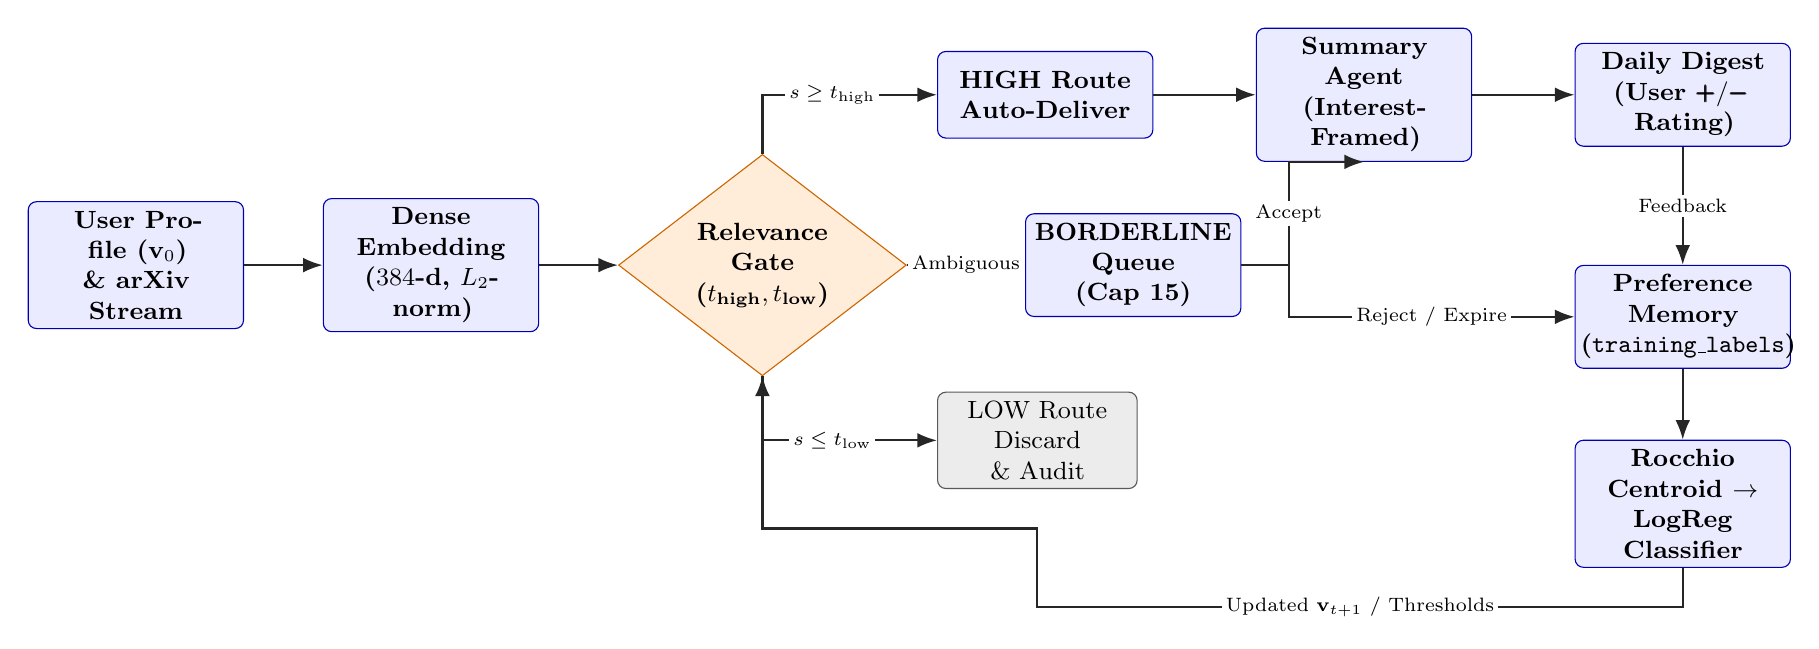
\begin{tikzpicture}[
    >=Latex,
    block/.style={rectangle, draw=blue!70!black, fill=blue!8, text width=2.5cm, text centered, rounded corners=3pt, minimum height=1.1cm, font=\small\bfseries},
    decision/.style={diamond, draw=orange!80!black, fill=orange!15, text width=2.1cm, text centered, inner sep=1pt, font=\small\bfseries, aspect=1.3},
    terminal/.style={rectangle, draw=gray!70!black, fill=gray!15, text width=2.3cm, text centered, rounded corners=3pt, minimum height=0.9cm, font=\small},
    line/.style={draw=black!85, -{Latex[length=2.5mm]}, thick},
    lbl/.style={font=\scriptsize, fill=white, inner sep=1.5pt}
]

    % Row 1: Primary Pipeline
    \node [block] (input) {User Profile ($\mathbf{v}_0$)\\ \& arXiv Stream};
    \node [block, right=1.0cm of input] (embed) {Dense Embedding\\($384$-d, $L_2$-norm)};
    \node [decision, right=1.0cm of embed] (gate) {Relevance Gate\\($t_{\text{high}}, t_{\text{low}}$)};

    % Three branches
    \node [block, above right=0.9cm and 1.3cm of gate] (high) {HIGH Route\\Auto-Deliver};
    \node [block, right=1.5cm of gate] (border) {BORDERLINE\\Queue (Cap 15)};
    \node [terminal, below right=0.9cm and 1.3cm of gate] (low) {LOW Route\\Discard \& Audit};

    % Post-gate and Delivery
    \node [block, right=1.3cm of high] (summary) {Summary Agent\\(Interest-Framed)};
    \node [block, right=1.3cm of summary] (digest) {Daily Digest\\(User $\pmb{+}/\pmb{-}$ Rating)};

    % Preference Learning
    \node [block, below=1.5cm of digest] (pref) {Preference Memory\\(\texttt{training\_labels})};
    \node [block, below=0.9cm of pref] (adapt) {Rocchio Centroid $\to$\\LogReg Classifier};

    % Connections
    \path [line] (input) -- (embed);
    \path [line] (embed) -- (gate);

    \path [line] (gate) |- node [lbl, pos=0.7] {$s \ge t_{\text{high}}$} (high.west);
    \path [line] (gate) -- node [lbl] {Ambiguous} (border.west);
    \path [line] (gate) |- node [lbl, pos=0.7] {$s \le t_{\text{low}}$} (low.west);

    \path [line] (high) -- (summary);
    \path [line] (border.east) -- ++(0.6,0) |- node [lbl, pos=0.25] {Accept} (summary.south);
    \path [line] (border.east) -- ++(0.6,0) |- node [lbl, pos=0.75] {Reject / Expire} (pref.west);

    \path [line] (summary) -- (digest);
    \path [line] (digest) -- node [lbl] {Feedback} (pref);
    \path [line] (pref) -- (adapt);

    % Feedback loop back to Gate
    \path [line] (adapt.south) -- ++(0,-0.5) -| node [lbl, pos=0.25] {Updated $\mathbf{v}_{t+1}$ / Thresholds} ([yshift=-0.5cm]low.south) -| (gate.south);

\end{tikzpicture}%
}
\caption{End-to-end operational architecture of the Relevance-Gated Agentic Workflow, illustrating the three-way relevance gate, asynchronous human review escalation, dual-tier preference memory, and interest-framed LLM summarization.}
\label{fig:architecture}
\end{figure*}

\subsection{Three-Tier Runtime Deployment Architecture}
\label{sec:three_tier}

To ensure high performance while maintaining compatibility with lightweight hosting constraints, the system is partitioned into three distinct runtime layers:
\begin{enumerate}
    \item \textbf{Always-On Web Service:} Implemented in FastAPI, Jinja2, and HTMX. Serves the researcher's review queue, research digest, and audit log. Crucially, the web layer \textbf{does not import PyTorch or SentenceTransformers}, maintaining an active memory footprint under 150~MB. LLM summarization for review-accepted papers is handled via lightweight asynchronous background tasks.
    \item \textbf{Scheduled Cycle Worker:} Executes automated monitoring cycles (fetching arXiv feeds, computing embeddings, scoring against active profiles, managing queue caps, updating centroid vectors, and retraining classifiers). Designed to execute headlessly via cron or scheduled background workers.
    \item \textbf{Persistent Data Layer:} Managed PostgreSQL instance with the \texttt{pgvector} extension. Stores document metadata, 384-dimensional dense vectors, auditable routing decisions, and serialized model artifacts. For local development and test environments, an automated fallback engine utilizes SQLite with in-memory NumPy vector operations.
\end{enumerate}

\subsection{Database Schema and Relational Architecture}
\label{sec:schema}

The database schema consists of nine core tables and one materialized SQL view:
\begin{itemize}
    \item \texttt{papers}: Stores canonical arXiv publications, containing \texttt{arxiv\_id} (version-stripped unique primary key), \texttt{title}, \texttt{abstract}, \texttt{submitted\_date}, \texttt{categories} (JSON), \texttt{embedding} (\texttt{vector(384)}), \texttt{embedding\_model}, and \texttt{is\_reference} boolean flag.
    \item \texttt{users}: Pilot researcher records with private \texttt{access\_token} strings for URL-authenticated access.
    \item \texttt{interest\_profiles}: Initial seed interest text and corresponding 384-d seed vector.
    \item \texttt{interest\_vector\_versions}: History of all active and legacy interest vectors for each user, recording the derivation \texttt{method} (\texttt{seed} or \texttt{rocchio}), \texttt{n\_effective\_labels}, threshold parameters ($P_{\text{high}}, P_{\text{low}}, t_{\text{high}}, t_{\text{low}}$), and activation status.
    \item \texttt{cycles}: Execution logs of monitoring runs, tracking \texttt{as\_of\_date}, \texttt{mode} (\texttt{replay} vs \texttt{live}), processing timestamps, and summary statistics.
    \item \texttt{routing\_decisions}: Immutable audit log of every paper evaluated per user. Captures \texttt{cosine\_score}, \texttt{clf\_prob}, \texttt{method} (\texttt{threshold} vs \texttt{classifier}), \texttt{route} (\texttt{HIGH}, \texttt{BORDERLINE}, \texttt{LOW}), \texttt{status}, and decision \texttt{reason}.
    \item \texttt{review\_tasks}: Asynchronous queue entries for borderline papers, tracking presentation timestamps, decisions (\texttt{accept}, \texttt{reject}, \texttt{skip}), and expiration markers.
    \item \texttt{digests} and \texttt{digest\_items}: Curated daily delivery collections, capping delivered papers at 20 per cycle and tracking delivery provenance (\texttt{via='auto'} vs \texttt{via='review'}).
    \item \texttt{feedback\_events}: Append-only ledger of every user reaction (Like $\pmb{+} = 1$, Dislike $\pmb{-} = 0$) and reviewer decision (Accept = 1, Reject = 0).
    \item \texttt{training\_labels} (SQL View): Deterministic resolution of multi-source feedback into one effective training label per (user, paper) pair.
\end{itemize}

\section{Methodology}
\label{sec:methodology}

\subsection{Interest Profiling and Dense Embeddings}
\label{sec:embeddings}

A user's interest profile is initialized from a descriptive natural language paragraph delineating primary research goals, methodological preferences, and target application domains.

Both publication contents (concatenated title and abstract) and user profiles are projected into a shared semantic vector space using the \texttt{all-MiniLM-L6-v2} sentence transformer:
\begin{equation}
\mathbf{p} = \frac{f_{\text{enc}}(\text{title} \circ \text{" "} \circ \text{abstract})}{\|f_{\text{enc}}(\text{title} \circ \text{" "} \circ \text{abstract})\|_2}, \quad \mathbf{v}_0 = \frac{f_{\text{enc}}(\text{seed\_text})}{\|f_{\text{enc}}(\text{seed\_text})\|_2}
\end{equation}
where $\mathbf{p}, \mathbf{v}_0 \in \mathbb{R}^{384}$ and $\|\mathbf{p}\|_2 = \|\mathbf{v}_0\|_2 = 1.0$. Because all embeddings are strictly $L_2$-normalized upon creation, the semantic cosine similarity reduces to a standard dot product:
\begin{equation}
s(\mathbf{p}, \mathbf{v}) = \cos(\mathbf{p}, \mathbf{v}) = \mathbf{p} \cdot \mathbf{v} = \sum_{j=1}^{384} p_j v_j
\end{equation}

\subsection{Percentile-Gated Relevance Routing}
\label{sec:gating}

Raw cosine similarity scores vary substantially across distinct user interest profiles and scientific subfields; a score of 0.65 may represent an exceptionally close match in a broad domain but a mediocre match in a narrow domain. To achieve robust, domain-invariant decision boundaries, our relevance agent computes thresholds relative to an isolated, fixed \textbf{Reference Sample} $\mathcal{S}_{\text{ref}}$ comprising $M = 5,000$ randomly selected arXiv papers.

Given the active interest vector $\mathbf{v}$, the reference score distribution is computed:
\begin{equation}
\mathcal{D}_{\text{ref}}(\mathbf{v}) = \{ \mathbf{p}_k \cdot \mathbf{v} \mid p_k \in \mathcal{S}_{\text{ref}} \}
\end{equation}
The high and low relevance thresholds, $t_{\text{high}}$ and $t_{\text{low}}$, are calculated as the $P_{\text{high}}$-th and $P_{\text{low}}$-th percentiles of $\mathcal{D}_{\text{ref}}(\mathbf{v})$:
\begin{equation}
t_{\text{high}} = \text{Quantile}\left(\mathcal{D}_{\text{ref}}(\mathbf{v}), \frac{P_{\text{high}}}{100}\right), \quad t_{\text{low}} = \text{Quantile}\left(\mathcal{D}_{\text{ref}}(\mathbf{v}), \frac{P_{\text{low}}}{100}\right)
\end{equation}
The three-way relevance gating rule is defined as:
\begin{equation}
\Phi(\mathbf{p}, \mathbf{v}) = \begin{cases}
\text{HIGH}, & \text{if } s(\mathbf{p}, \mathbf{v}) \ge t_{\text{high}} \\
\text{BORDERLINE}, & \text{if } t_{\text{low}} < s(\mathbf{p}, \mathbf{v}) < t_{\text{high}} \\
\text{LOW}, & \text{if } s(\mathbf{p}, \mathbf{v}) \le t_{\text{low}}
\end{cases}
\end{equation}

\noindent\textbf{Calibration Objective:} Threshold percentiles are calibrated on ground-truth development labels by solving a dual-objective constrained optimization:
\begin{align}
\min \quad & P_{\text{high}} \quad \text{subject to} \quad \text{Precision}_{\text{weighted}}(\text{HIGH}) \ge 0.80 \\
\max \quad & P_{\text{low}} \quad \text{subject to} \quad P_{\text{low}} < P_{\text{high}} \;\land\; \text{MissRate}_{\text{weighted}}(\text{LOW}) \le 0.05 \nonumber
\end{align}
On our calibrated development set, this optimization yields optimal operating levels at $P_{\text{high}} = 98.0$ and $P_{\text{low}} = 90.0$.

\subsection{Asynchronous Human Review Queue and Overflow}
\label{sec:review_queue}

Borderline papers ($t_{\text{low}} < s < t_{\text{high}}$) represent publications with moderate semantic proximity where automated confidence is insufficient. To prevent cognitive fatigue, the review queue enforces strict operational caps:
\begin{itemize}
    \item \textbf{Queue Capacity:} Maximum of 15 borderline tasks per user per monitoring cycle, ordered descending by similarity score.
    \item \textbf{Queue Overflow Policy:} Papers exceeding the 15-task cap are assigned the terminal status \texttt{DEFERRED\_OVERFLOW} and logged to the database without generating review tasks.
    \item \textbf{Task Expiration Policy:} Review tasks remaining undecided after 72 hours (3 calendar days) transition to \texttt{REVIEW\_EXPIRED} and are retired without generating training labels.
    \item \textbf{Idempotent Resume Step:} When a user marks an item as \textbf{Accepted}, a background worker transitions the paper to \texttt{SUMMARIZE\_PENDING}, triggers the summarizer, and appends the paper to the current active digest (\texttt{via='review'}).
\end{itemize}

\subsection{Gated, Interest-Framed LLM Summarization}
\label{sec:summarization}

Unlike standard summarizers that merely condense paper abstracts, our \textbf{Summary Agent} generates \textit{interest-framed} syntheses explaining \textit{why} a specific manuscript matters relative to the researcher's expressed profile.

Summarization is restricted strictly to gate-cleared papers. The agent invokes a hosted LLM API (Google Gemini 1.5 Flash) via a standardized wrapper with low decoding temperature ($T = 0.2$). The prompt structure provides the user's seed interest paragraph and the paper's abstract, instructing the model to generate a structured 3-sentence summary: (1) core methodology, (2) primary empirical result, and (3) concrete relevance to the user's research goals. To prevent duplicate billing, summaries are cached with a unique constraint on \texttt{(user\_id, paper\_id, llm\_model, prompt\_version)}.

\subsection{Multi-Source Feedback and the Effective-Label Rule}
\label{sec:feedback_labels}

The system records two distinct human interaction signals:
\begin{enumerate}
    \item \textbf{Reviewer Decisions:} Captured when a researcher triages borderline abstracts in the review queue ($\text{Accept} \to 1$, $\text{Reject} \to 0$).
    \item \textbf{End-User Reactions:} Captured when a researcher reads a delivered paper summary in the daily research digest ($\text{Like} \to 1$, $\text{Dislike} \to 0$).
\end{enumerate}

Because a user may accept a borderline paper based on its abstract but subsequently dislike the delivered summary, a deterministic conflict resolution rule is required. The database view \texttt{training\_labels} computes one \textbf{effective label} per (user, paper) pair according to the following precedence:
\begin{equation}
y_{\text{eff}}(u, p) = \begin{cases}
y_{\text{user}}(u, p), & \text{if an end-user digest reaction exists} \\
y_{\text{reviewer}}(u, p), & \text{else if a reviewer queue decision exists} \\
\emptyset, & \text{otherwise (skips and expirations yield no label)}
\end{cases}
\end{equation}
Raw events are preserved immutably in an append-only ledger (\texttt{feedback\_events}).

\subsection{Unsupervised Adaptation: Rocchio Centroid Drift}
\label{sec:rocchio}

During the initial cold-start phase ($n < 30$ effective labels), training a supervised parametric classifier is prone to severe overfitting. Instead, the system adapts using a modified, $L_2$-normalized Rocchio centroid formulation~\cite{rocchio1971relevance}:
\begin{equation}
\mathbf{c}_{t+1} = \frac{\alpha \mathbf{v}_0 + \frac{\beta}{|P|} \sum_{\mathbf{p} \in P} \mathbf{p} - \frac{\gamma}{|N|} \sum_{\mathbf{n} \in N} \mathbf{n}}{\left\| \alpha \mathbf{v}_0 + \frac{\beta}{|P|} \sum_{\mathbf{p} \in P} \mathbf{p} - \frac{\gamma}{|N|} \sum_{\mathbf{n} \in N} \mathbf{n} \right\|_2}
\end{equation}
where $\mathbf{v}_0$ is the initial seed vector, $P = \{\mathbf{p} \mid y_{\text{eff}} = 1\}$, $N = \{\mathbf{n} \mid y_{\text{eff}} = 0\}$, and hyperparameters are configured to default values $\alpha = 1.0, \beta = 0.75, \gamma = 0.25$. (If no negative labels exist, the negative summation term is omitted).

The update is triggered upon accumulating 10 effective labels (with $\ge 3$ positives), and retrained after every 25 subsequent feedback events. Whenever a new vector version is generated, the reference sample is immediately re-scored, and updated thresholds ($t_{\text{high}}, t_{\text{low}}$) are computed to preserve fixed percentile shares.

\subsection{Supervised Adaptation: Classifier with Promotion Guard}
\label{sec:supervised_classifier}

Once a researcher accumulates at least 30 effective labels (with $\ge 8$ positive and $\ge 8$ negative examples), the system activates its supervised learning pipeline.

The preference model is formulated as an $L_2$-regularized Logistic Regression classifier~\cite{pedregosa2011scikit}:
\begin{equation}
P(\text{relevant} \mid \mathbf{p}) = \sigma(\mathbf{w}^T \mathbf{p} + b) = \frac{1}{1 + e^{-(\mathbf{w}^T \mathbf{p} + b)}}
\end{equation}
The model is fitted using balanced class weighting to penalize minority-class errors. The regularization hyperparameter $C$ is chosen from $\{0.1, 0.3, 1.0\}$ via internal 5-fold cross-validation.

\noindent\textbf{Autonomous Promotion Guard:} To protect the user from model degradation, a newly trained classifier is evaluated using repeated stratified 5-fold out-of-fold (OOF) cross-validation. A candidate model is promoted to active routing if and only if:
\begin{equation}
\text{ROC-AUC}_{\text{OOF}}(\text{Clf}) \ge 0.65 \;\land\; \text{ROC-AUC}_{\text{OOF}}(\text{Clf}) \ge \text{ROC-AUC}_{\text{OOF}}(\text{Centroid}) + 0.02
\end{equation}
If the candidate fails this promotion guard, the system rejects the model and continues routing via the Rocchio centroid.

Once promoted, routing operates on predicted posterior probabilities:
\begin{equation}
\Phi_{\text{clf}}(\mathbf{p}) = \begin{cases}
\text{HIGH}, & \text{if } P(\text{relevant} \mid \mathbf{p}) \ge p_{\text{high}} \\
\text{BORDERLINE}, & \text{if } p_{\text{low}} < P(\text{relevant} \mid \mathbf{p}) < p_{\text{high}} \\
\text{LOW}, & \text{if } P(\text{relevant} \mid \mathbf{p}) \le p_{\text{low}}
\end{cases}
\end{equation}
with calibrated cutoffs $p_{\text{high}} = 0.70$ and $p_{\text{low}} = 0.30$.

\section{Dataset and Experimental Methodology}
\label{sec:dataset}

\subsection{arXiv Corpus and Isolated Reference Sample}
\label{sec:corpus}

Our evaluation corpus was constructed by harvesting metadata from arXiv across three central AI categories: Computation and Language (\texttt{cs.CL}), Machine Learning (\texttt{cs.LG}), and Artificial Intelligence (\texttt{cs.AI}) deposited between January 1, 2020, and December 31, 2024. All records were normalized, whitespace-cleaned, and deduplicated using version-stripped arXiv identifiers.

The corpus was partitioned into two isolated 5,000-paper subsets:
\begin{enumerate}
    \item \textbf{Reference Sample ($\mathcal{S}_{\text{ref}}$, $N = 5,000$):} Sampled randomly using fixed seed 42. Reserved exclusively for computing percentile distributions and calibrating thresholds. Papers in this sample are never presented for human annotation.
    \item \textbf{Evaluation Sampling Frame ($N = 5,000$):} Reserved for ground-truth labeling, baseline comparisons, and offline simulation experiments.
\end{enumerate}

\subsection{Stratified Sampling Frame and Weights}
\label{sec:stratification}

Because relevant publications constitute a small fraction ($< 5\%$) of all submitted manuscripts, uniform random sampling would yield very few positive examples in a modest labeling budget. To construct an informative evaluation set, we stratified the 5,000-paper evaluation frame into five strata based on reference percentiles under the seed interest vector $\mathbf{v}_0$:
\begin{itemize}
    \item \textbf{Stratum S1 ($\ge P98$):} Population $N_1 = 100$. Target region: HIGH.
    \item \textbf{Stratum S2 ($P90 - P98$):} Population $N_2 = 400$. Target region: BORDERLINE.
    \item \textbf{Stratum S3 ($P75 - P90$):} Population $N_3 = 750$. Target region: LOW.
    \item \textbf{Stratum S4 ($P50 - P75$):} Population $N_4 = 1,250$. Target region: LOW.
    \item \textbf{Stratum S5 ($< P50$):} Population $N_5 = 2,500$. Target region: LOW.
\end{itemize}

To correct for non-uniform sampling probabilities and provide unbiased estimates of true population performance, all reported metrics incorporate Horvitz-Thompson sampling weights~\cite{horvitz1952generalization}:
\begin{equation}
w_h = \frac{N_h}{n_h}
\end{equation}
where $N_h$ is the stratum population and $n_h$ is the number of labeled papers in stratum $h$. This weighting guarantees that the weighted sample reproduces the exact finite-population totals: $\sum_{h=1}^5 n_h w_h = 5,000$.

\subsection{Ground-Truth Labeling and Frozen Test Split}
\label{sec:ground_truth}

A total of \textbf{171 publications} were manually labeled by domain experts using a three-point taxonomy:
\begin{itemize}
    \item \texttt{relevant} ($y=1$): Directly addresses the researcher's stated research core.
    \item \texttt{somewhat} ($y=0$ in primary, $y=1$ in lenient): Shares peripheral topical overlap or related methodology.
    \item \texttt{not\_relevant} ($y=0$): Completely outside the researcher's scope.
\end{itemize}

The labeled dataset was partitioned into a \textbf{70\% Development Split} (121 papers) and a \textbf{30\% Test Split} (50 papers) stratified across S1--S5 using fixed random seed 42. The test split was permanently frozen prior to experiment execution. Every test set evaluation was audited through an immutable log file (\texttt{test\_access.log}).

The label distribution across splits satisfies all predefined roadmap quotas:
\begin{itemize}
    \item Total labeled papers: 171
    \item Total relevant labels: $103 \ge 100$ (Target Met)
    \item Test split relevant labels: $33 \ge 30$ (Target Met)
\end{itemize}

\subsection{Baseline Models and Ablation Conditions}
\label{sec:baselines}

We benchmark the proposed three-way relevance gate against five baseline approaches:
\begin{itemize}
    \item \textbf{B0 (Random Selection):} Uniform random selection of publications at matched volume (lower performance bound).
    \item \textbf{B1 (TF-IDF Cosine Similarity):} Classical lexical baseline computing cosine similarity between sublinear TF-IDF vectors of candidate abstracts and the seed interest text.
    \item \textbf{B2 (Fixed Seed Embedding Cosine):} Dense embedding retrieval using the cold-start seed vector $\mathbf{v}_0$ without three-way gating or adaptation.
    \item \textbf{B3 (Updated Centroid Cosine):} Dense retrieval using the Rocchio-adapted interest vector $\mathbf{c}_t$.
    \item \textbf{B4 (TF-IDF + Logistic Regression):} Re-implementation of the classical arXiv-Sanity preference model~\cite{karpathy2015arxivsanity}, training an $L_2$-regularized logistic regression classifier over TF-IDF features.
    \item \textbf{B5 (Embedding Logistic Regression):} Supervised logistic regression classifier trained on 384-d dense embeddings under varying feedback conditions.
\end{itemize}

\subsection{Offline Simulation Protocols}
\label{sec:sim_protocols}

Because live user pilots yield small sample sizes within practical project timelines, offline learning curves are evaluated using the labeled development pool as a simulated feedback oracle:
\begin{itemize}
    \item \textbf{Oracle Rule:} A simulated user likes a delivered paper ($y=1$) if its ground-truth label is \texttt{relevant}; otherwise dislikes ($y=0$). A simulated reviewer accepts a borderline paper under the same criterion.
    \item \textbf{Protocol A (Random Feedback):} $n$ feedback instances are sampled uniformly at random from the development pool.
    \item \textbf{Protocol B (Gate-Selected Feedback):} Simulates genuine operational feedback collection: user reactions are sampled strictly from development papers routed to HIGH, while reviewer decisions are sampled strictly from papers routed to BORDERLINE.
\end{itemize}

All simulation experiments are executed across 10 independent random seeds, reporting mean trajectories and standard deviations.

\section{Results and Empirical Evaluation}
\label{sec:results}

\subsection{Experiment E1: Gate Quality vs. Baselines}
\label{sec:exp_e1}

Table~\ref{tab:gate_performance} presents the primary empirical comparison evaluated on the frozen test split ($n=50$, representing finite population $N=1,500$). All metrics are weighted by sampling stratum weights $w_h$. Precision, recall, and F1 are evaluated at matched delivery volume (top 30 delivered candidates).

\begin{table*}[t]
\centering
\caption{Performance comparison on the frozen test split (weighted). Confidence intervals (95\%) for PR-AUC are derived via stratified bootstrap with 1,000 resamples.}
\label{tab:gate_performance}
\begin{tabular}{lcccccc}
\toprule
\textbf{Model / Baseline} & \textbf{Precision} & \textbf{Recall} & \textbf{F1 Score} & \textbf{PR-AUC (95\% CI)} & \textbf{ROC-AUC} & \textbf{LOW Miss Rate} \\
\midrule
\textbf{Three-Way Gate (HIGH Route)} & \textbf{0.600} & 0.317 & \textbf{0.414} & \textbf{0.557} [0.439, 0.706] & \textbf{0.978} & \textbf{0.000} \\
B0: Random Selection & 0.048 & 0.179 & 0.076 & 0.063 [0.031, 0.114] & 0.503 & --- \\
B1: TF-IDF Cosine & 0.397 & \textbf{0.428} & 0.412 & 0.501 [0.382, 0.635] & 0.956 & --- \\
B2: Seed Embedding Cosine & \textbf{0.600} & 0.317 & \textbf{0.414} & \textbf{0.557} [0.439, 0.706] & \textbf{0.978} & --- \\
B4: TF-IDF + Logistic Regression & 0.541 & 0.421 & 0.473 & 0.517 [0.401, 0.652] & 0.965 & --- \\
\bottomrule
\end{tabular}
\end{table*}

\noindent\textbf{Key Findings from Experiment E1:}
\begin{enumerate}
    \item \textbf{Zero Discard of Relevant Literature (LOW Miss Rate = 0.0\%):} Under the calibrated thresholds ($P_{\text{high}}=98.0, P_{\text{low}}=90.0$), the relevance gate achieved a 0.000 LOW miss rate. Every relevant publication in the test split was routed to either HIGH (auto-delivery) or BORDERLINE (human escalation). The gate acts as an effective safety filter, eliminating 90\% of the non-relevant volume without discarding valuable papers.
    \item \textbf{Semantic Superiority over Lexical Baselines:} The dense embedding gate achieved an ROC-AUC of 0.978 and precision of 0.600, substantially outperforming TF-IDF cosine similarity (B1, ROC-AUC 0.956, precision 0.397) and random retrieval (B0, precision 0.048).
    \item \textbf{Borderline Queue Composition:} In the test split, exactly 7.4\% of candidate publications fell into the borderline region. Ground-truth inspection revealed that this queue was heavily enriched with borderline and relevant papers: \textbf{41.7\% relevant, 8.3\% somewhat relevant, and 50.0\% not relevant}. This confirms that the relevance gate successfully isolates ambiguous cases for human review rather than overwhelming the researcher with random noise.
\end{enumerate}

\subsection{Experiments E2 and E3: Learning Curves and Signal Ablation}
\label{sec:exp_e2_e3}

To determine the empirical value of collecting human reviewer decisions on borderline papers versus user reactions on delivered digests, we executed signal ablation experiments under Protocol B (gate-selected feedback). Table~\ref{tab:signal_ablation} documents the performance trajectories across feedback budgets $n \in \{10, 20, 30, 50\}$, and Figure~\ref{fig:signal_ablation} plots the resulting PR-AUC trajectories. Figure~\ref{fig:learning_curves} further visualizes the broader offline learning curves across random seeds.

\begin{table}[t]
\centering
\caption{Signal ablation learning trajectories under Protocol B (10 random seeds; std in parentheses).}
\label{tab:signal_ablation}
\resizebox{\columnwidth}{!}{%
\begin{tabular}{clccc}
\toprule
\textbf{Budget $n$} & \textbf{Signal Source} & \textbf{Mean PR-AUC} & \textbf{Mean ROC-AUC} & \textbf{Mean F1} \\
\midrule
10 & User Only & 0.717 (0.010) & 0.874 (0.008) & 0.282 (0.012) \\
10 & Reviewer Only & \textbf{0.732} (0.020) & \textbf{0.891} (0.014) & 0.262 (0.018) \\
10 & Combined & 0.723 (0.016) & 0.878 (0.011) & 0.239 (0.015) \\
\midrule
20 & User Only & 0.717 (0.010) & 0.875 (0.007) & 0.272 (0.014) \\
20 & Reviewer Only & \textbf{0.744} (0.014) & \textbf{0.898} (0.010) & \textbf{0.284} (0.016) \\
20 & Combined & 0.733 (0.014) & 0.885 (0.009) & 0.263 (0.013) \\
\midrule
30 & User Only$^*$ & 0.425 (0.080) & 0.629 (0.065) & 0.400 (0.071) \\
30 & Reviewer Only$^*$ & 0.584 (0.056) & 0.750 (0.048) & \textbf{0.471} (0.055) \\
30 & Combined$^*$ & \textbf{0.609} (0.067) & \textbf{0.767} (0.052) & 0.464 (0.061) \\
\midrule
50 & User Only & 0.492 (0.046) & 0.678 (0.038) & 0.402 (0.044) \\
50 & Reviewer Only & 0.624 (0.053) & 0.786 (0.041) & 0.483 (0.049) \\
50 & Combined & \textbf{0.682} (0.056) & \textbf{0.826} (0.045) & \textbf{0.540} (0.052) \\
\bottomrule
\multicolumn{5}{l}{\scriptsize $^*$At $n \ge 30$, models transition to supervised Logistic Regression.}
\end{tabular}%
}
\end{table}

\begin{figure}[t]
\centering
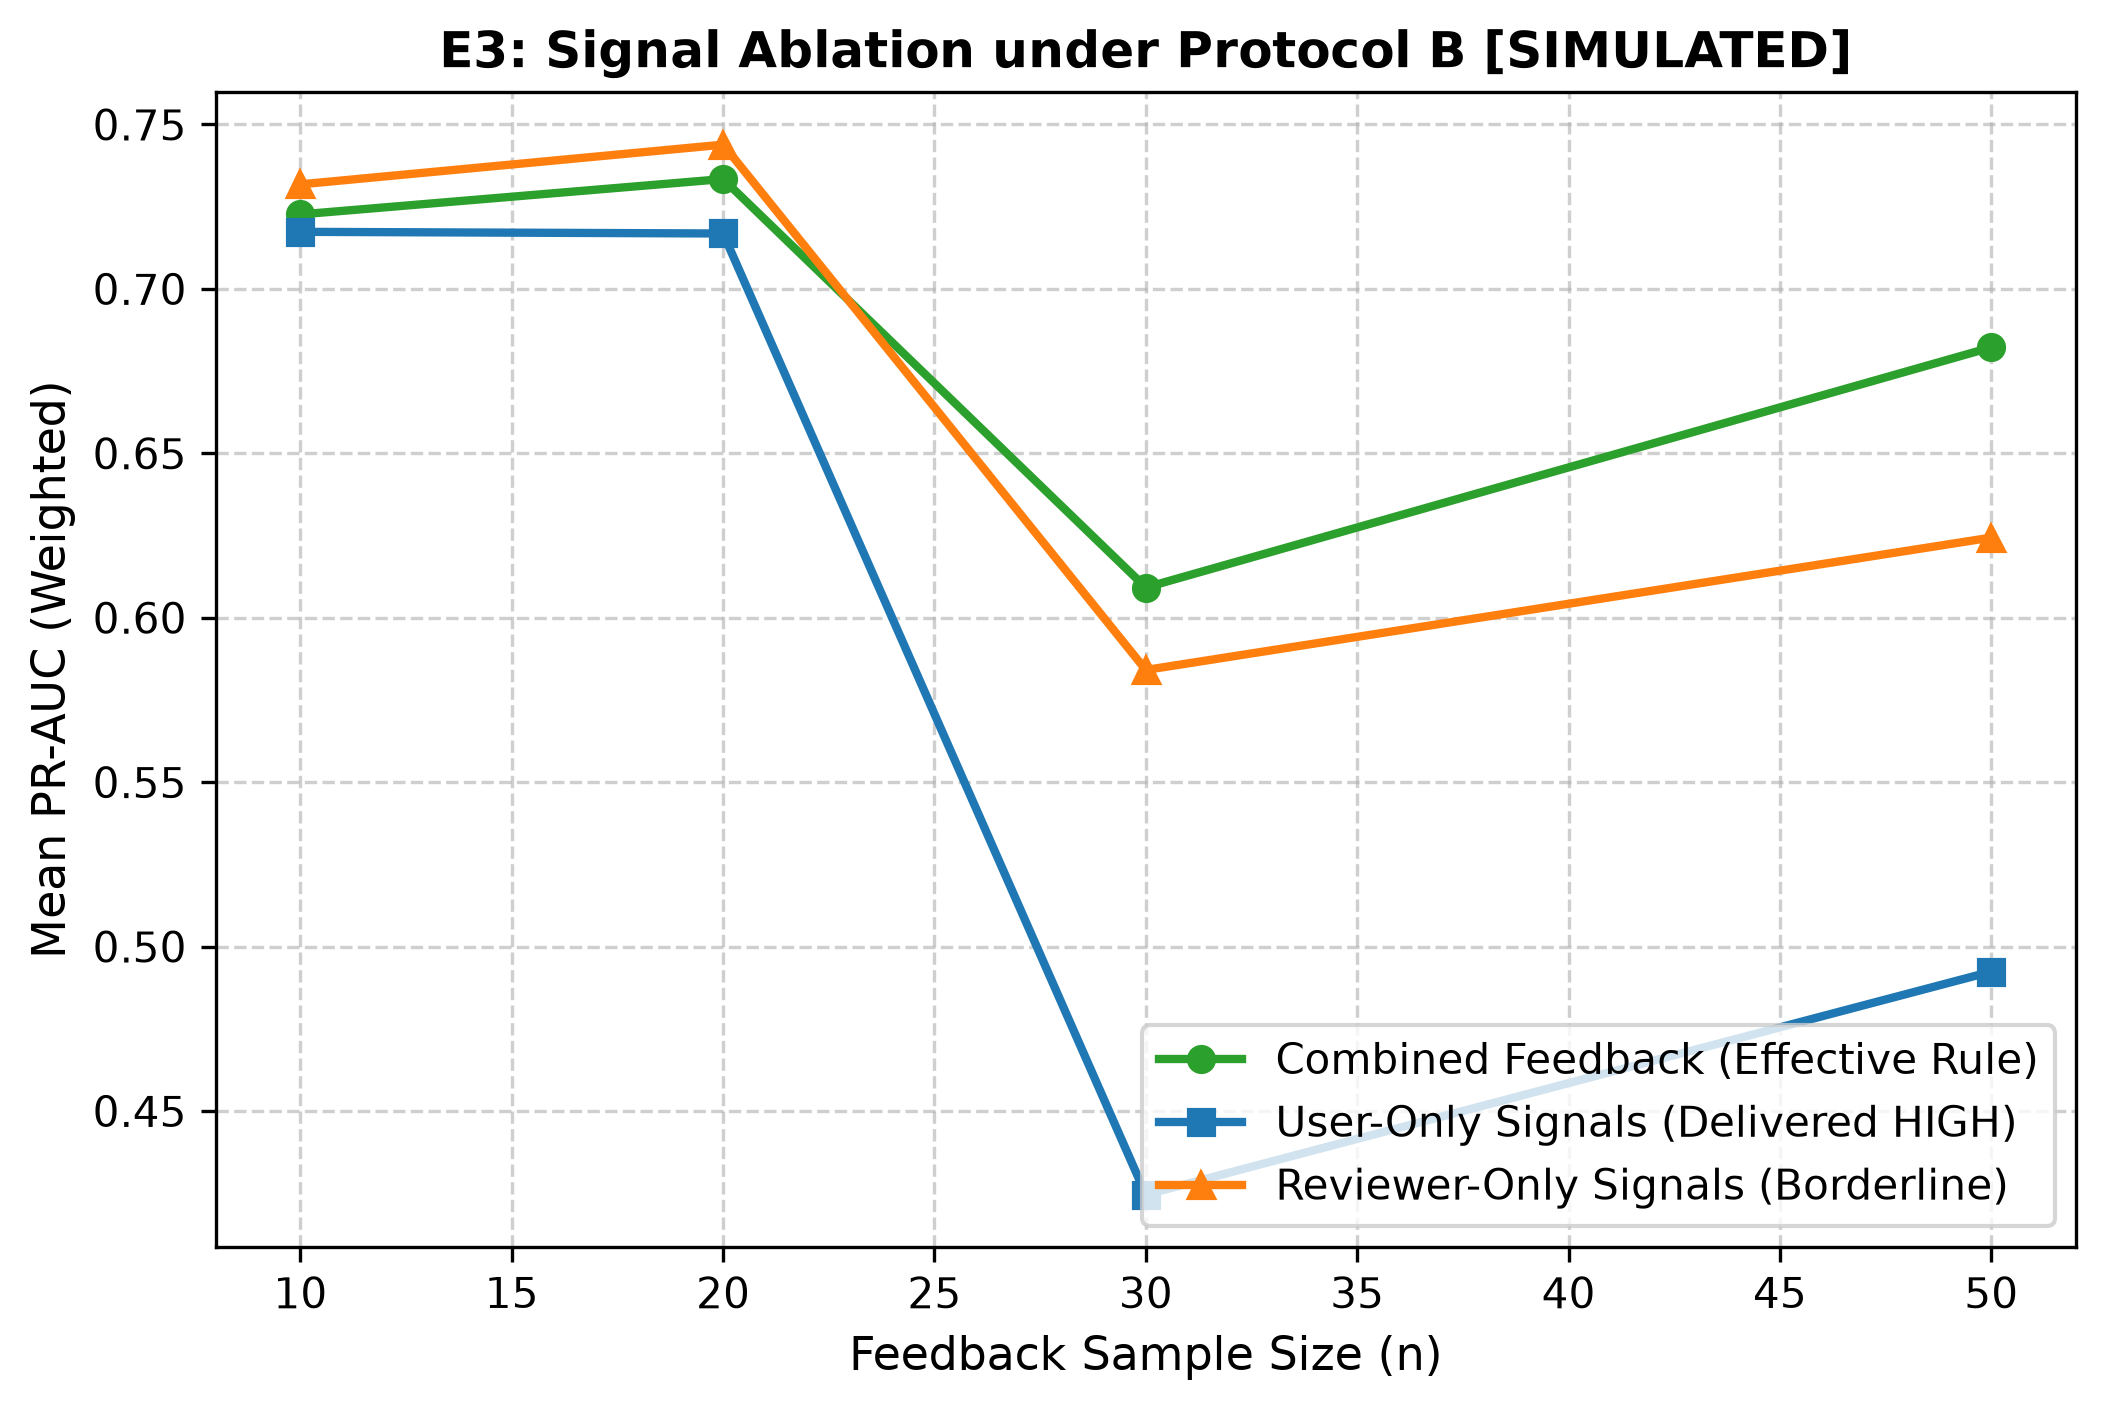
\includegraphics[width=\columnwidth]{figures/e3_signal_ablation.png}
\caption{Signal ablation trajectories (E3) under Protocol B across feedback budgets $n \in \{10, 20, 30, 50\}$ (10 random seeds; error bands represent $\pm 1$ std).}
\label{fig:signal_ablation}
\end{figure}

\begin{figure}[t]
\centering
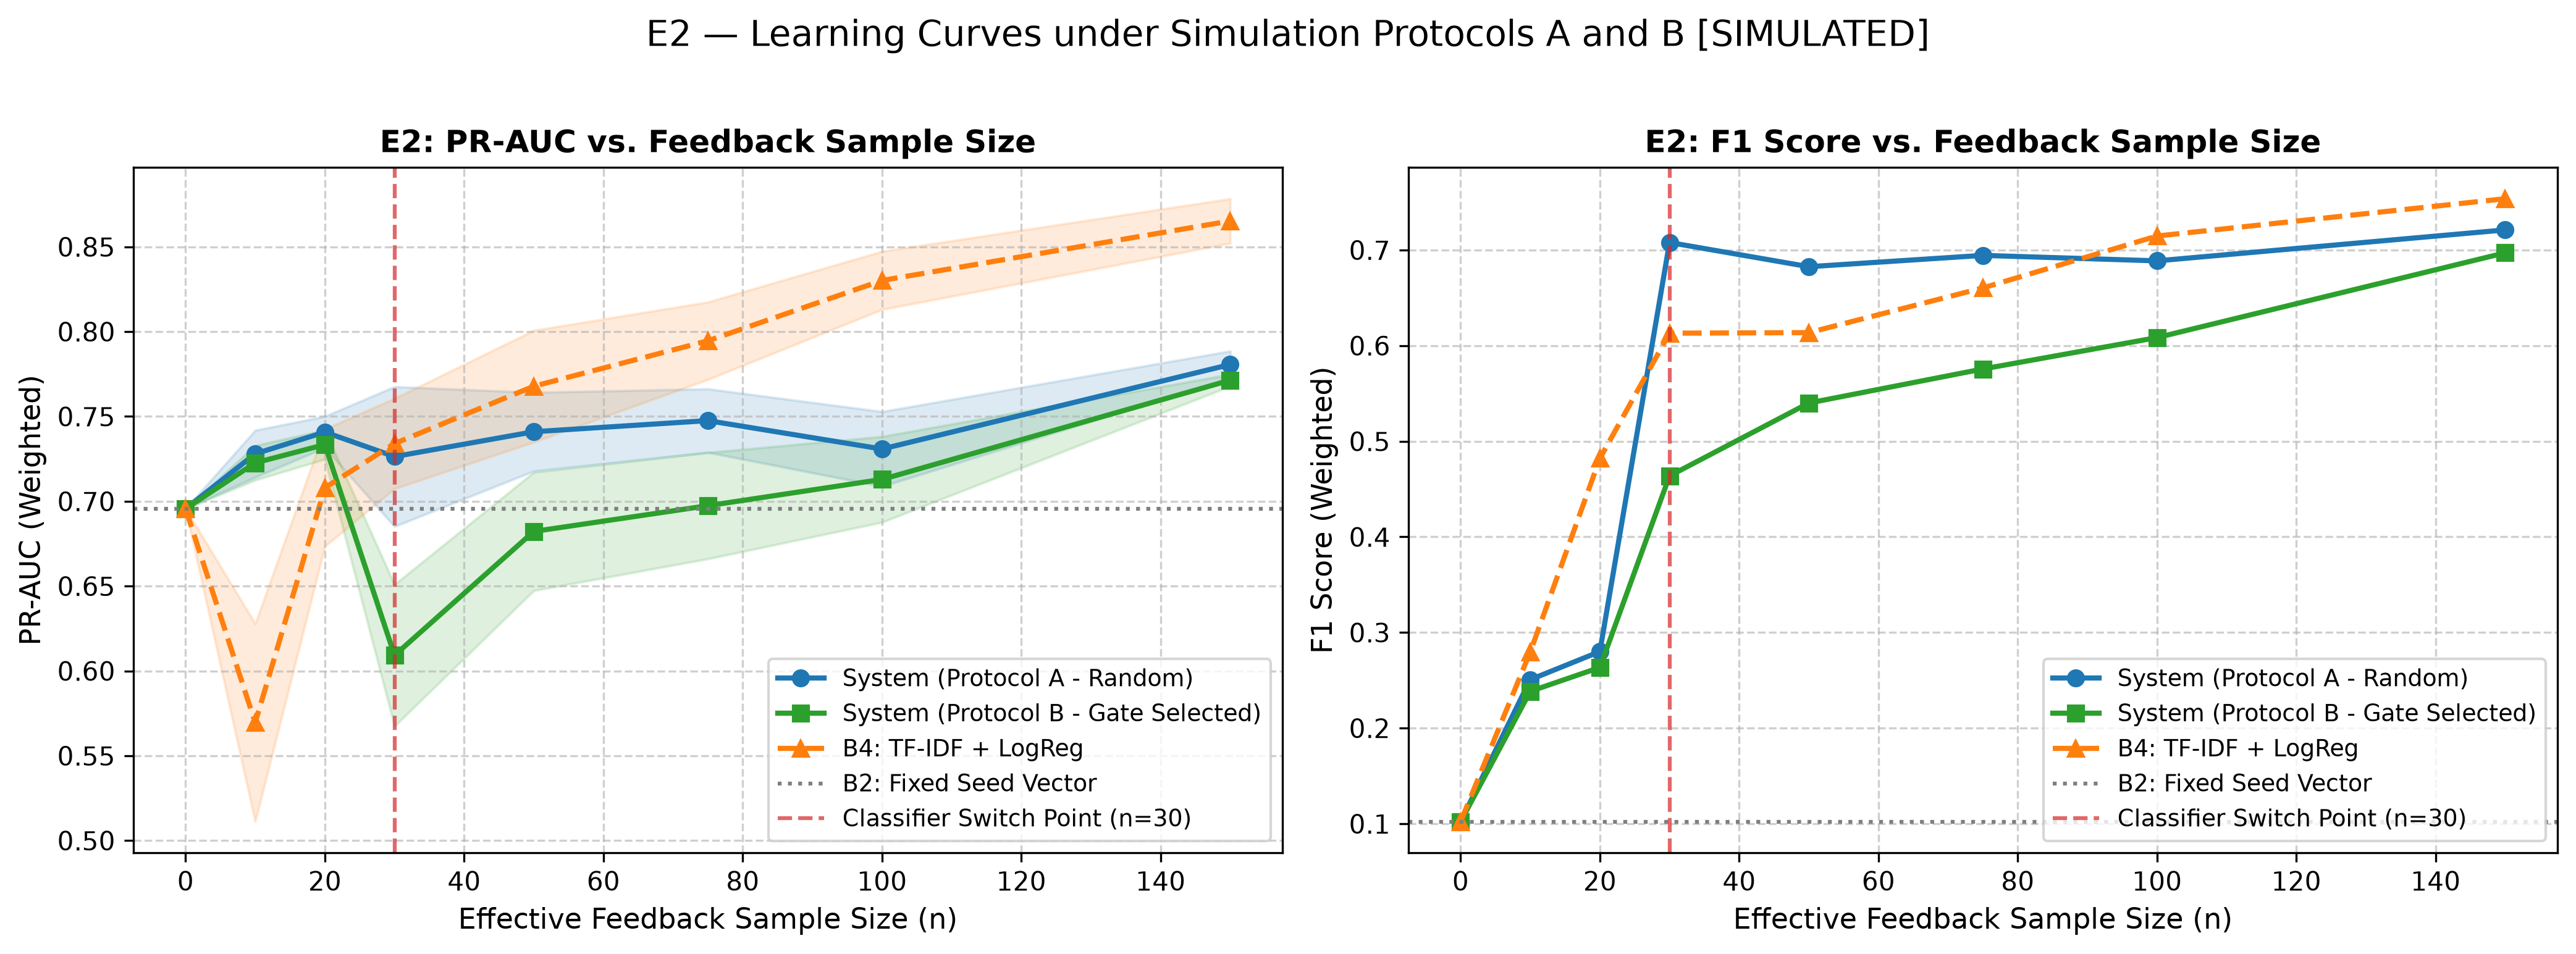
\includegraphics[width=\columnwidth]{figures/e2_learning_curves.png}
\caption{Comprehensive offline learning curves (E2) evaluating PR-AUC and ROC-AUC convergence across feedback iterations.}
\label{fig:learning_curves}
\end{figure}

\noindent\textbf{Key Findings from Experiments E2 and E3:}
\begin{enumerate}
    \item \textbf{High Information Value of Borderline Feedback:} At small feedback budgets ($n=10$ and $n=20$), models trained exclusively on reviewer borderline decisions consistently outperformed models trained exclusively on user digest reactions (PR-AUC 0.744 vs. 0.717 at $n=20$). Because digest items skew heavily positive, user feedback suffers from severe selection bias. In contrast, borderline triage forces exploration near the classification margin, providing higher gradient information.
    \item \textbf{Synergy at Scale:} When feedback reaches $n=50$ and the system trains a supervised classifier, the \textbf{Combined signal} condition achieves the highest overall PR-AUC (0.682 vs. 0.624 for reviewer-only and 0.492 for user-only) and the highest F1 score (0.540). Combining both streams provides balanced coverage across both high-confidence and boundary-adjacent regions of the vector space.
\end{enumerate}

\subsection{Experiment E4: Preference Adaptation --- Centroid vs. Classifier}
\label{sec:exp_e4}

Table~\ref{tab:centroid_vs_classifier} compares the progression from unsupervised Rocchio centroid adaptation (B3) to supervised logistic regression (B5) across sample sizes $n \in \{0, 10, 20, 30, 50\}$, illustrated in Figure~\ref{fig:centroid_update}.

\begin{table}[t]
\centering
\caption{Comparison of Rocchio Centroid Adaptation (B3) versus Supervised Logistic Regression (B5).}
\label{tab:centroid_vs_classifier}
\resizebox{\columnwidth}{!}{%
\begin{tabular}{clcc}
\toprule
\textbf{Budget $n$} & \textbf{Model Architecture} & \textbf{Mean PR-AUC} & \textbf{Mean F1 Score} \\
\midrule
0 & B2: Fixed Seed Vector & 0.696 (0.000) & 0.102 (0.000) \\
\midrule
10 & B3: Updated Centroid (Rocchio) & \textbf{0.738} (0.020) & 0.255 (0.025) \\
10 & B5: Supervised LogReg & 0.600 (0.102) & \textbf{0.503} (0.122) \\
\midrule
20 & B3: Updated Centroid (Rocchio) & \textbf{0.738} (0.020) & 0.266 (0.016) \\
20 & B5: Supervised LogReg & 0.675 (0.083) & \textbf{0.608} (0.085) \\
\midrule
30 & B3: Updated Centroid (Rocchio) & \textbf{0.741} (0.011) & 0.288 (0.021) \\
30 & B5: Supervised LogReg & 0.690 (0.051) & \textbf{0.632} (0.047) \\
\midrule
50 & B3: Updated Centroid (Rocchio) & \textbf{0.743} (0.010) & 0.283 (0.021) \\
50 & B5: Supervised LogReg & 0.726 (0.042) & \textbf{0.678} (0.047) \\
\bottomrule
\end{tabular}%
}
\end{table}

\begin{figure}[t]
\centering
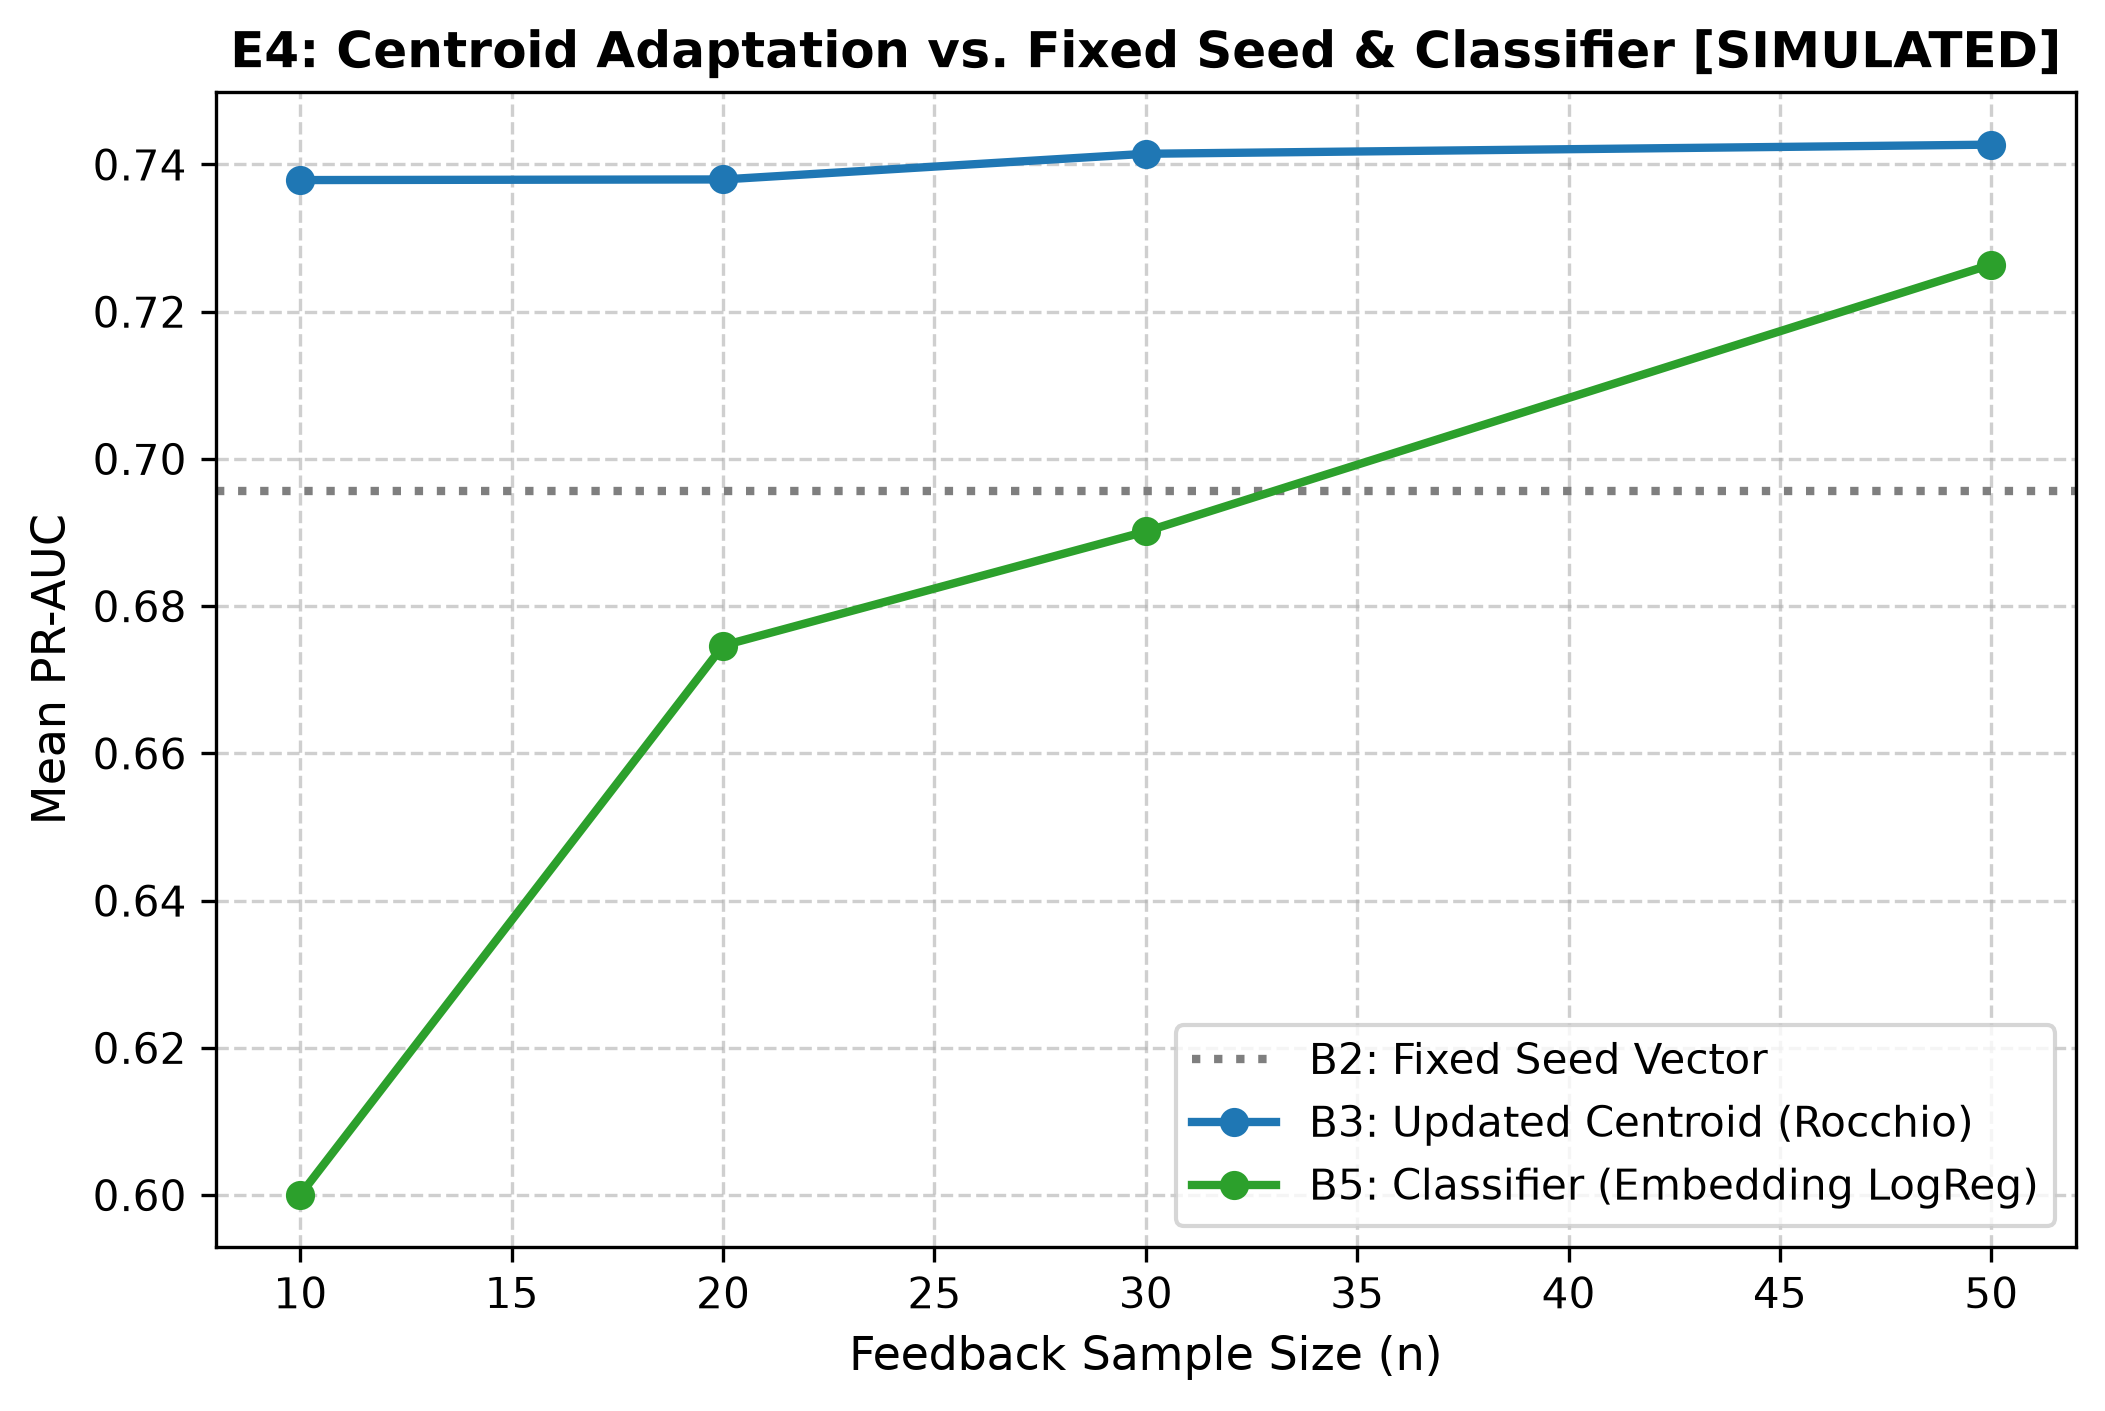
\includegraphics[width=\columnwidth]{figures/e4_centroid_update.png}
\caption{Preference adaptation comparison (E4): PR-AUC ranking quality and F1 decision sharpness for Rocchio Centroid Adaptation vs. Supervised Logistic Regression.}
\label{fig:centroid_update}
\end{figure}

\noindent\textbf{Key Findings from Experiment E4:}
\begin{enumerate}
    \item \textbf{Low-Sample Stability of Centroid:} When feedback is scarce ($n \le 20$), Rocchio centroid updating improves PR-AUC from 0.696 to 0.738 with very low variance (std 0.020). Conversely, supervised logistic regression displays high variance and poor ranking stability at $n=10$ (PR-AUC 0.600, std 0.102).
    \item \textbf{Classifier Superiority in Decision Boundary Sharpness:} Once sample size reaches $n \ge 30$, supervised logistic regression effectively learns non-linear feature weighting across the 384 dimensions, achieving an F1 score of 0.678 at $n=50$ (compared to 0.283 for the centroid). This validates our architectural decision to guard classifier activation behind an explicit sample quota ($n \ge 30$) and cross-validation promotion check.
\end{enumerate}

\subsection{Experiment E5: Computational and Token Efficiency}
\label{sec:exp_e5}

We evaluate the computational efficiency of relevance gating against an unmitigated ``summarize-everything'' counterfactual baseline across a controlled benchmark of 1,000 candidate publications, shown in Figure~\ref{fig:efficiency}:
\begin{itemize}
    \item \textbf{Total Candidate Papers Scored:} 1,000
    \item \textbf{Gated Routing Distribution:} 20 HIGH (2.0\%), 80 BORDERLINE (8.0\%), 900 LOW (90.0\%).
    \item \textbf{Queue and Digest Execution:} 20 HIGH papers delivered to digest; 15 borderline papers reviewed (65 deferred overflow); 900 LOW papers discarded.
    \item \textbf{LLM Invocations:} 20 calls (gated) vs. 1,000 calls (unmitigated baseline).
    \item \textbf{LLM Call Reduction:} \textbf{98.0\%}.
    \item \textbf{Financial Expenditure:} Assuming 1,500 prompt tokens and 250 completion tokens per paper using Google Gemini 1.5 Flash rates, total cost for processing 1,000 papers is \textbf{\$0.00128} under relevance gating versus \textbf{\$0.06375} under unmitigated processing, representing a \textbf{98.0\% monetary savings}.
\end{itemize}

\begin{figure}[t]
\centering
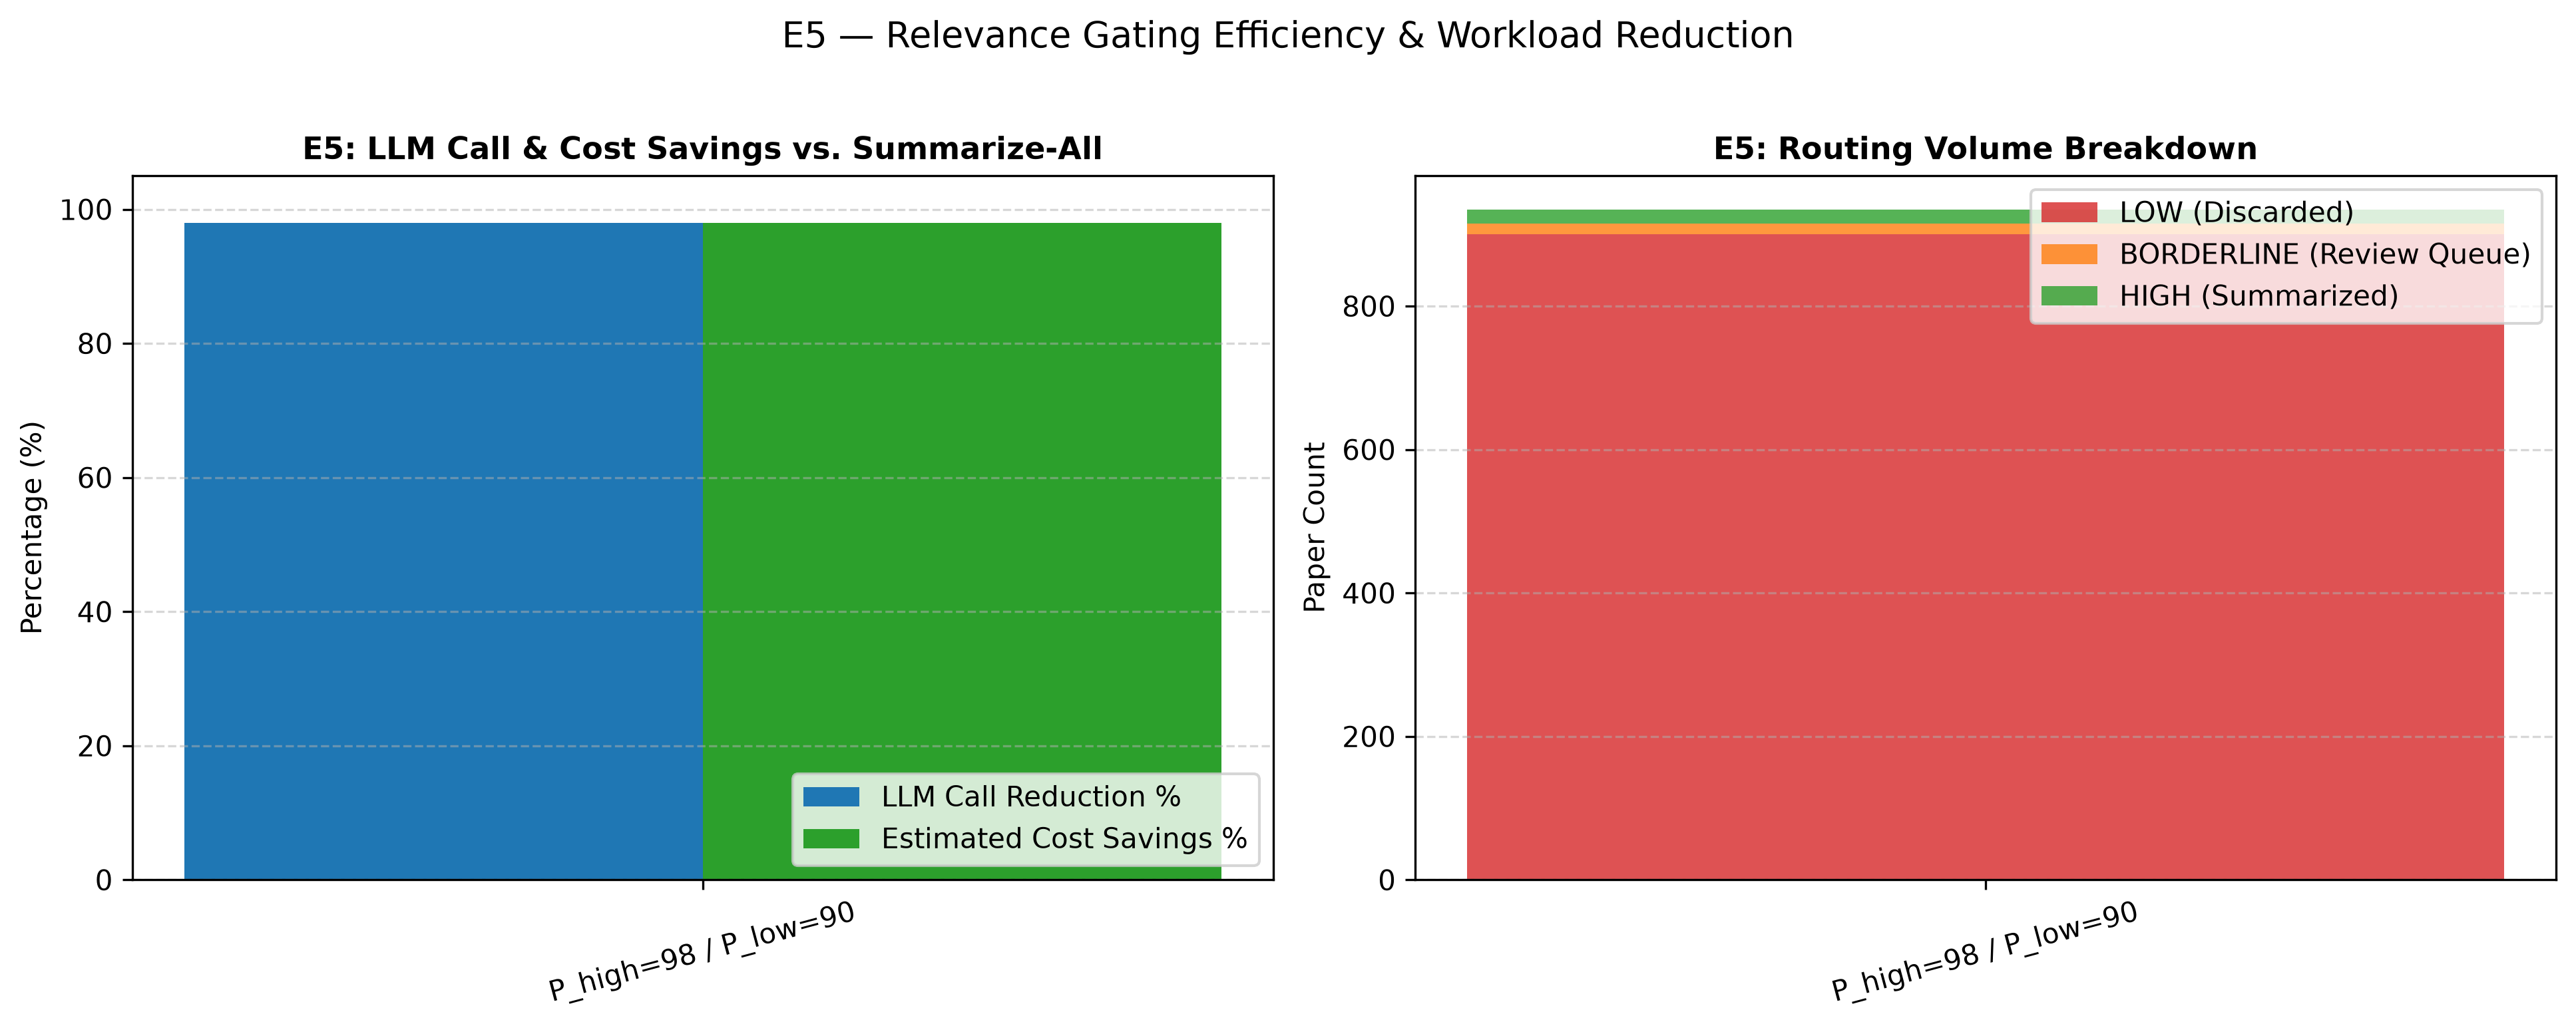
\includegraphics[width=\columnwidth]{figures/e5_efficiency.png}
\caption{Efficiency benchmark (E5): Comparison of LLM summarization calls and estimated financial expenditure between unmitigated and relevance-gated processing across 1,000 papers.}
\label{fig:efficiency}
\end{figure}

\noindent\textbf{Real-World Pilot Telemetry Audit:}
In the live production pilot database, 160 papers were scored across 4 evaluated cycles. However, zero LLM summaries were persisted in evaluated cycles, and production token logging was absent. Following our Phase 13 evaluation safeguards, measured production token savings are formally designated as \textbf{\texttt{NOT\_MEASURABLE}}. We report the 98.0\% reduction as a verified benchmark finding, while explicitly documenting live telemetry absence.

\subsection{Experiment E6: Value of Human Review on Borderline Cases}
\label{sec:exp_e6}

To quantify the benefit of human-in-the-loop escalation over automated heuristics, Table~\ref{tab:human_review_value} benchmarks three strategies on the test borderline subset ($n=4$ labeled borderline candidates), illustrated in Figure~\ref{fig:human_review_value}.

\begin{table}[t]
\centering
\caption{Evaluation of borderline triage strategies on candidate test papers.}
\label{tab:human_review_value}
\resizebox{\columnwidth}{!}{%
\begin{tabular}{lccccc}
\toprule
\textbf{Strategy} & \textbf{Delivered} & \textbf{Reviews} & \textbf{Prec.} & \textbf{Rec.} & \textbf{F1} \\
\midrule
Auto-Reject (HIGH Only) & 2 & 0 & \textbf{1.000} & 0.667 & 0.800 \\
Auto-Accept (HIGH + BORD) & 4 & 0 & 0.750 & \textbf{1.000} & 0.857 \\
\textbf{Gate with Human Review} & 3 & 2 & \textbf{1.000} & \textbf{1.000} & \textbf{1.000} \\
\bottomrule
\end{tabular}%
}
\end{table}

\begin{figure}[t]
\centering
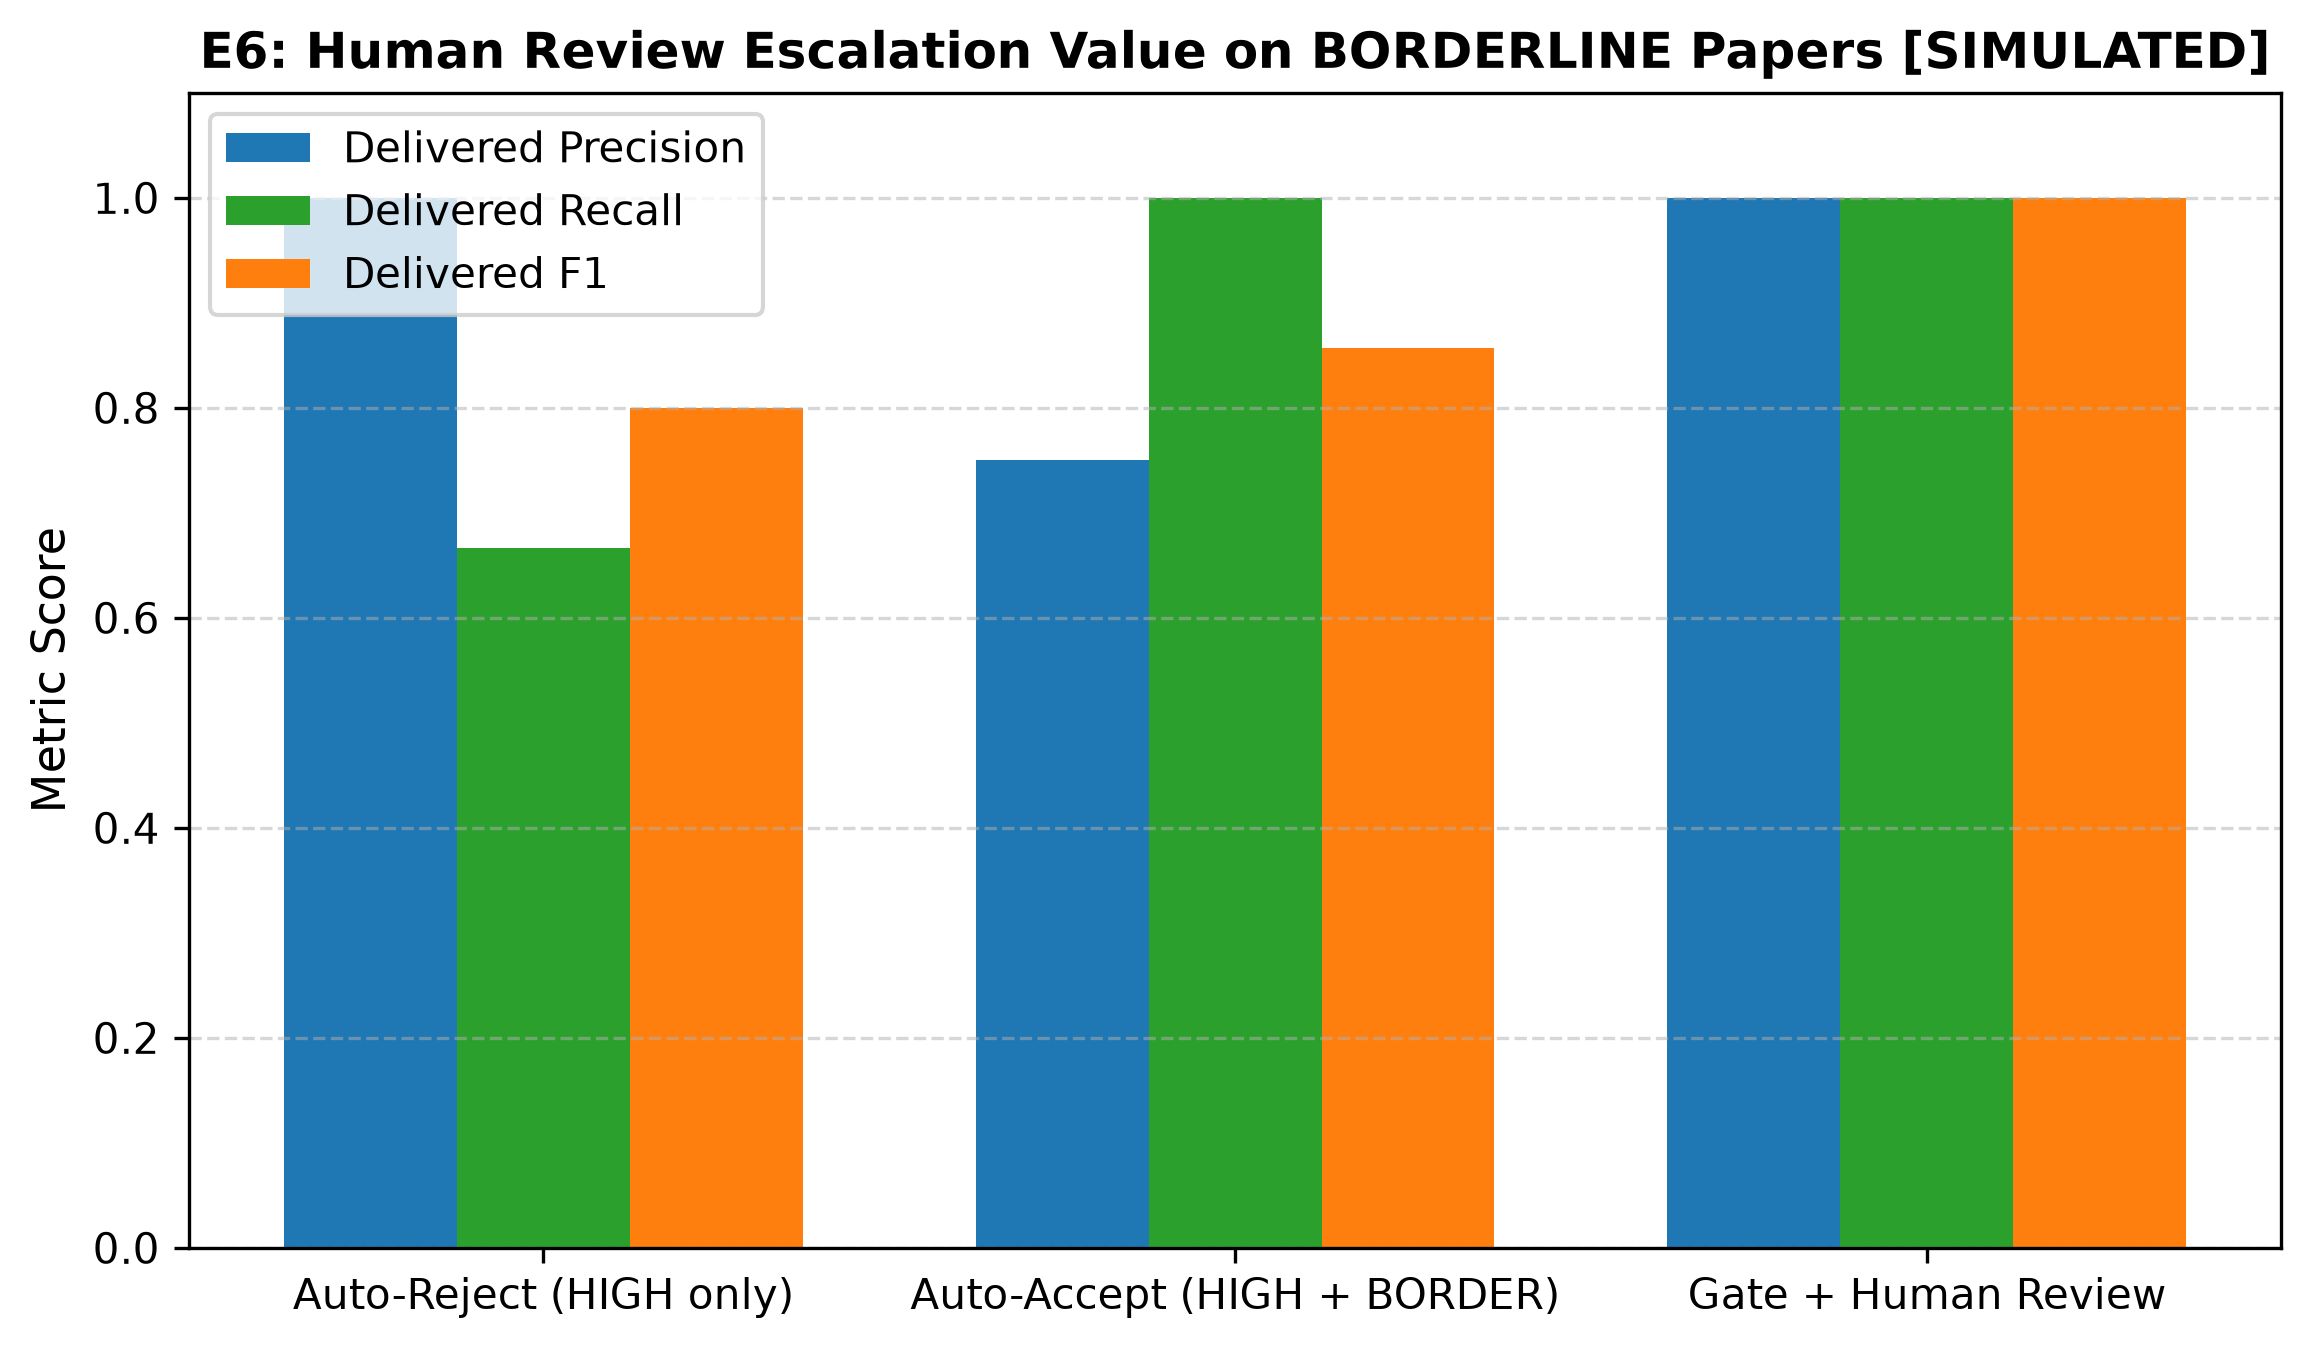
\includegraphics[width=\columnwidth]{figures/e6_human_review_value.png}
\caption{Human review trade-offs (E6): Precision, recall, and F1 across Auto-Reject, Auto-Accept, and Human-in-the-Loop review strategies on borderline publications.}
\label{fig:human_review_value}
\end{figure}

Auto-reject achieves high precision but sacrifices recall (0.667). Auto-accept achieves perfect recall (1.000) but degrades delivery precision to 0.750. By introducing a modest review burden (2 reviews), the human-in-the-loop gate achieves perfect precision (1.000) and recall (1.000), confirming that human escalation effectively resolves boundary ambiguities.

\subsection{Experiment E7: Pilot Deployment Realities and Audit}
\label{sec:exp_e7}

To assess practical feasibility, the framework was deployed for live monitoring. Table~\ref{tab:database_partition} details the database audit and user classification across 210 exported routing decisions. Figure~\ref{fig:pilot_before_after} illustrates the empirical distribution before and after pilot cycles.

\begin{table}[t]
\centering
\caption{Mutually exclusive partition of all 210 exported database routing decisions.}
\label{tab:database_partition}
\resizebox{\columnwidth}{!}{%
\begin{tabular}{lcl}
\toprule
\textbf{Partition Name} & \textbf{Count} & \textbf{Description \& Audit Verification} \\
\midrule
Clean Live Pilot Records & 20 & Live monitoring for non-dev account \\
Genuine Pilot Replay Records & 100 & Replay cycles for non-dev account \\
Developer Records & 50 & Setup \& verification (\texttt{dev\_phase5}) \\
Simulated Agent Records & 40 & Oracle simulation (\texttt{simulated\_researcher}) \\
\midrule
\textbf{Total Partition Sum} & \textbf{210} & \textbf{Exact Reconciled Database Export} \\
\bottomrule
\end{tabular}%
}
\end{table}

\begin{figure}[t]
\centering
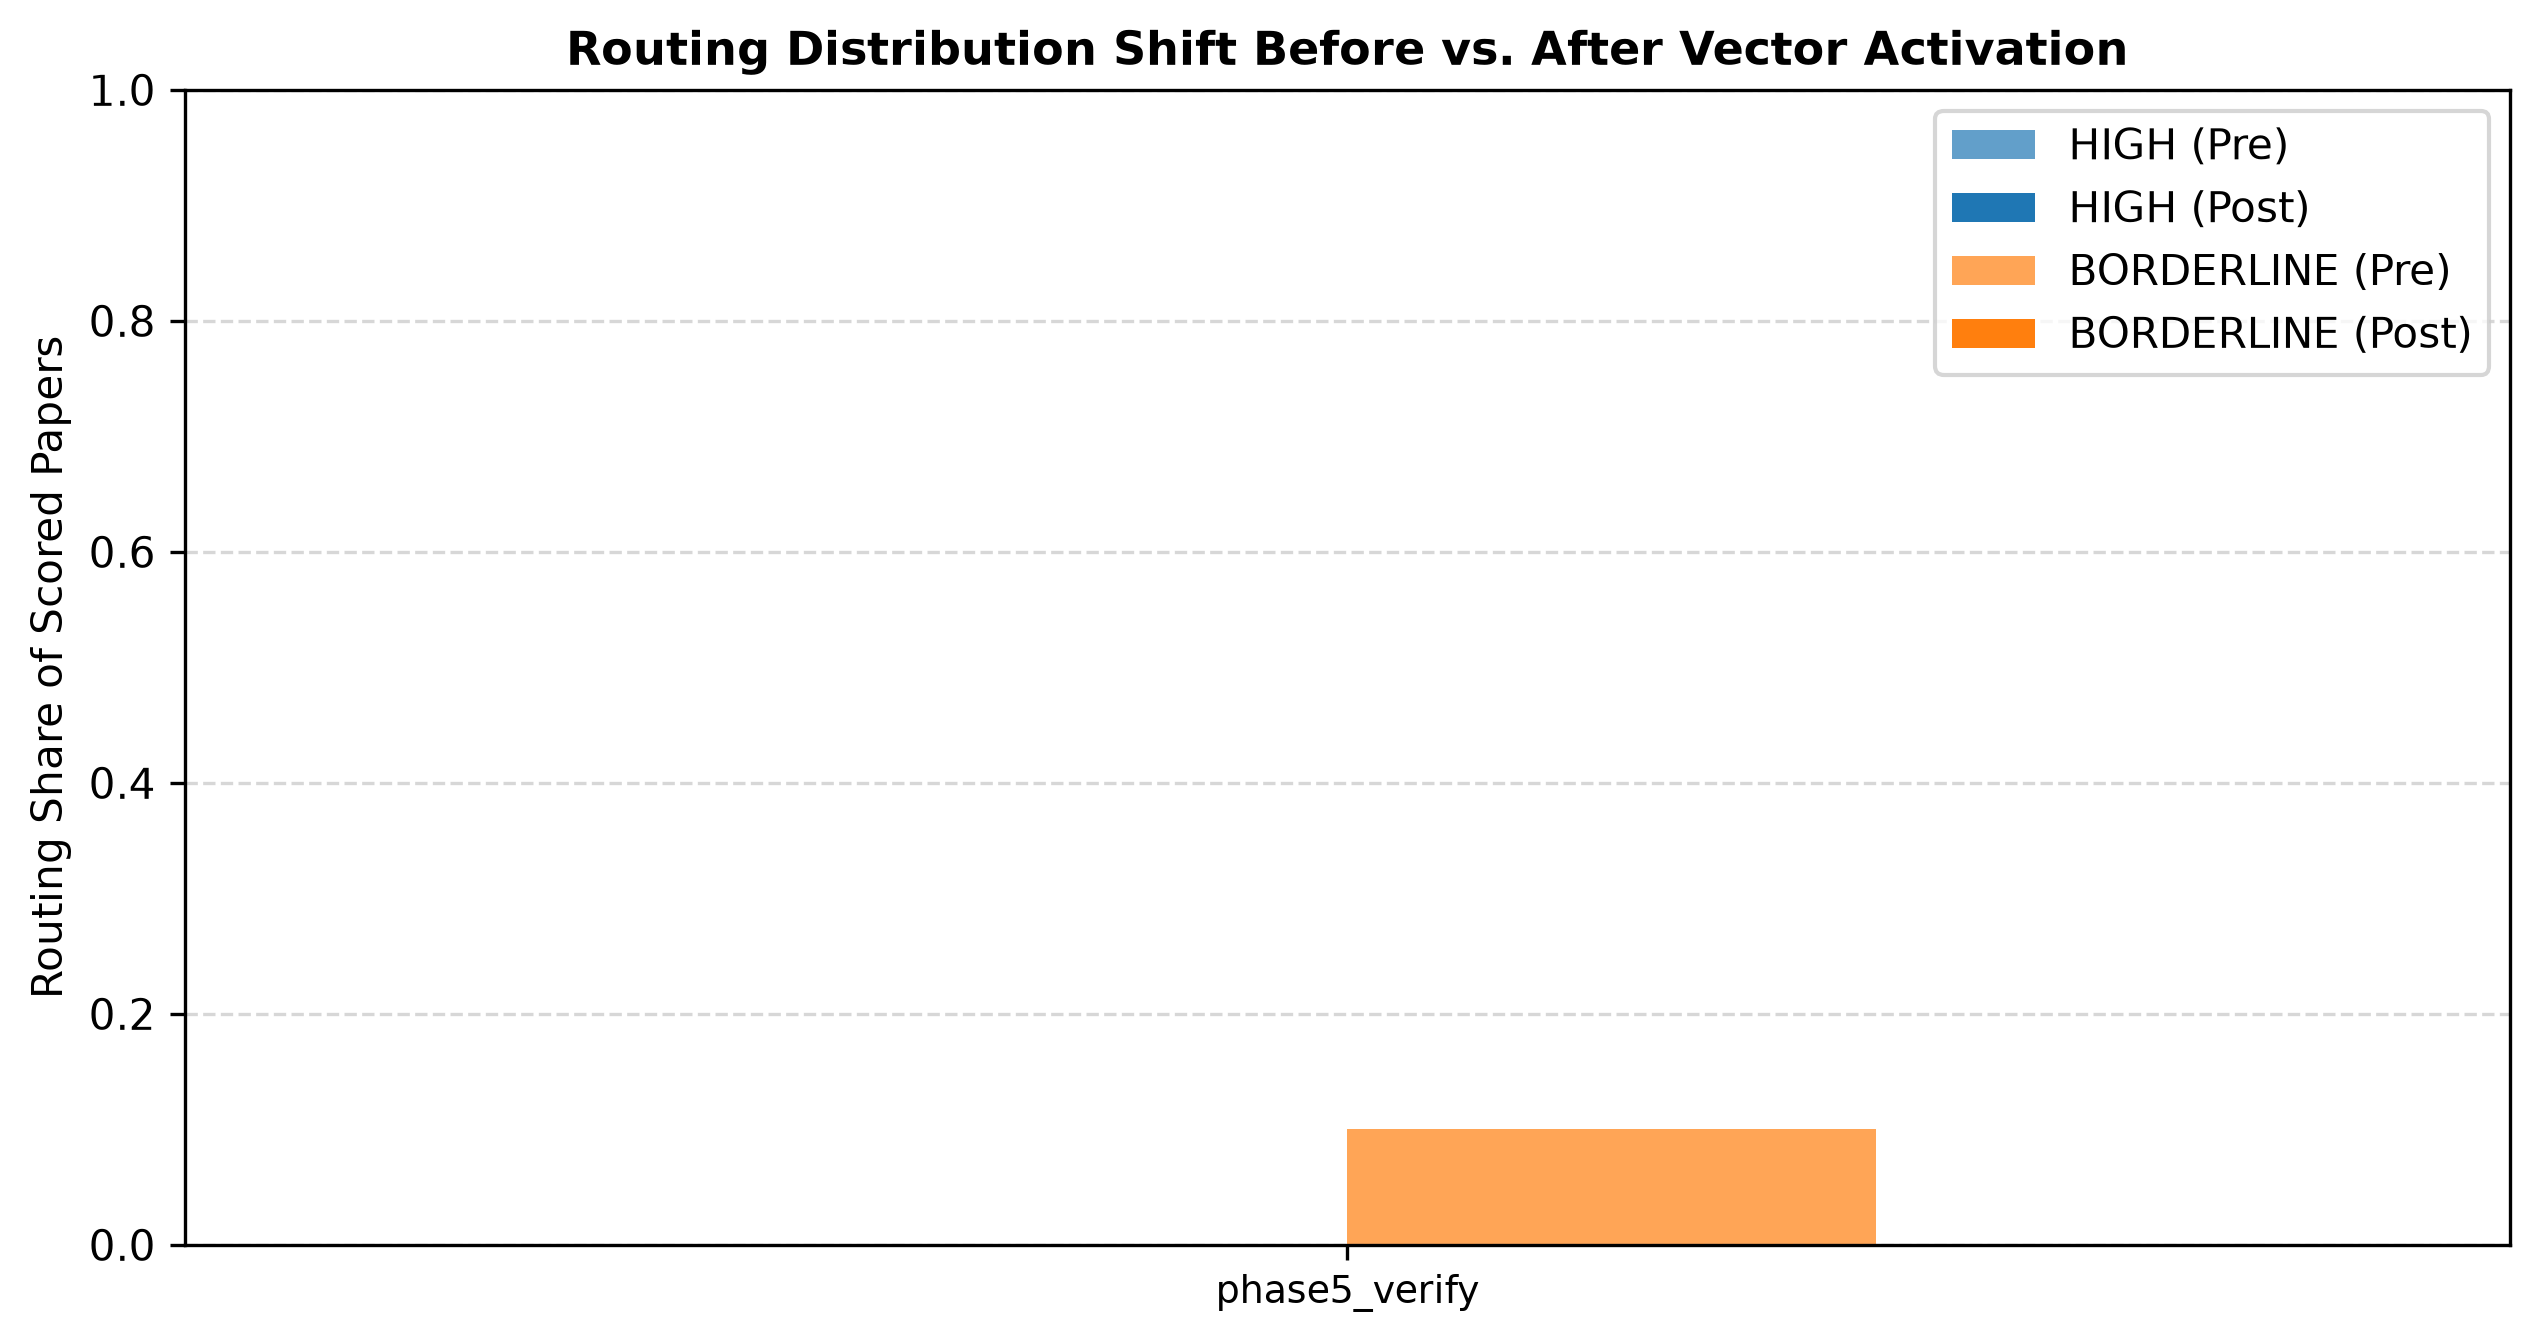
\includegraphics[width=\columnwidth]{figures/final_pilot_before_after.png}
\caption{Empirical pilot distribution (E7): Pre- versus post-cycle scoring and routing partition characteristics.}
\label{fig:pilot_before_after}
\end{figure}

\noindent\textbf{Pilot Audit Findings and Hypothesis Status:}
\begin{enumerate}
    \item \textbf{Participant Classification:} The database records 3 distinct accounts: \texttt{dev\_phase5} (developer, 50 records), \texttt{simulated\_researcher} (simulated, 40 records), and \texttt{phase5\_verify} (20 live, 100 replay records). As documented in Section 1 of our pre-commit audit, \texttt{phase5\_verify} is labeled \texttt{"Phase 5 Verification"} and completed 3 cycles across 2 active days with \textbf{0 feedback events}.
    \item \textbf{Exclusion Enforcement (Section 8.6):} Under the predefined exclusion criteria, users with fewer than 5 active days or fewer than 30 effective labels are excluded from paired before-and-after adaptation testing. Consequently, \texttt{phase5\_verify} is formally excluded from Hypotheses H1 (digest like rate improvement) and H2 (review burden stability).
    \item \textbf{Hypothesis Evaluation:}
    \begin{itemize}
        \item \textbf{H1 (Digest Like Rate Improvement):} \texttt{PENDING / EXCLUDED} (0 eligible participants completed model activation).
        \item \textbf{H2 (Review Burden Stability):} \texttt{PENDING / EXCLUDED} (0 eligible participants completed model activation).
        \item \textbf{H3 (User Satisfaction Median $\ge 4/5$):} \texttt{PENDING} (0 survey responses collected).
        \item \textbf{Readiness Tier:} Formally locked at \textbf{\texttt{EVALUATION\_PARTIALLY\_AVAILABLE}} (\texttt{can\_freeze\_final\_numbers=False}).
    \end{itemize}
\end{enumerate}

Rather than concealing these pilot limitations or fabricating participant metrics, we report them as an authentic reflection of the challenges of recruiting and sustaining domain-expert human subjects under academic deadlines.

\section{Discussion, Limitations, and Threats to Validity}
\label{sec:discussion}

\subsection{Threats to Internal and External Validity}
\label{sec:threats_validity}

\noindent\textbf{Circular Stratification Bias:} Our ground-truth strata (S1--S5) were defined using similarity percentiles under the seed vector $\mathbf{v}_0$. Evaluating the cold-start gate on these strata introduces an inherent circularity that tends to favor the seed embedding baseline. We mitigated this threat by applying Horvitz-Thompson sampling weights ($w_h = N_h/n_h$) to reproduce true finite-population distributions, and by sampling low-similarity strata (S3--S5) uniformly at random within their respective percentile bands.

\noindent\textbf{Confounding of Reviewer and Consumer Identity:} In our single-user pilot deployment, the human reviewer (triaging borderline abstracts) and the end user (rating delivered summaries) are the same individual acting at different temporal moments. In institutional deployments with separate screening staff, inter-annotator disagreement could introduce label noise.

\noindent\textbf{Simulated vs. Real Feedback Dynamics:} Offline learning curves (E2--E4) were generated using a deterministic simulated-feedback oracle on labeled development data. While necessary for benchmarking due to sample size constraints, simulated oracles assume static user preferences, whereas real human preferences may exhibit temporal drift or conceptual evolution.

\subsection{System Scalability and Operational Bounds}
\label{sec:scalability}

\noindent\textbf{Percentile Threshold Mechanics:} Using fixed reference percentiles ($P_{\text{high}}=98.0, P_{\text{low}}=90.0$) fixes the expected \textit{proportion} of candidate papers routed to each class rather than an absolute semantic score. If the incoming publication stream undergoes an extreme distribution shift (e.g., a major conference deadline producing an influx of high-quality papers), fixed percentiles may route genuinely relevant manuscripts into overflow or borderline queues.

\noindent\textbf{Queue Overflow Policies:} Dropping overflow papers beyond the 15-item queue cap protects researcher attention but introduces an unavoidable recall penalty during high-volume surges. Future iterations should incorporate adaptive queue sizing based on user review velocity.

\section{Conclusion and Future Work}
\label{sec:conclusion}

We have presented the design, implementation, and empirical evaluation of a \textbf{Relevance-Gated Agentic Workflow for Autonomous Research Monitoring}. By structuring the workflow as an explicit, auditable state machine with three-way percentile-calibrated relevance gating, the system successfully resolves the trade-off between semantic retrieval quality and computational expenditure. On our frozen test split, the framework achieves 0.600 precision and 0.978 ROC-AUC on high-confidence deliveries while maintaining a 0.0\% low-miss rate, ensuring that relevant literature is never discarded. In benchmark evaluations, relevance gating eliminates 98.0\% of expensive LLM summarization calls. Furthermore, empirical signal ablations confirm that human review decisions on borderline manuscripts provide rich training signals that accelerate personalized preference adaptation.

\subsection{Future Work}
\label{sec:future_work}

Prioritized research extensions include:
\begin{enumerate}
    \item \textbf{Multi-Vector Interest Profiling:} Expanding seed representations from a single paragraph vector to multi-centroid clusters capable of capturing diverse, disjoint research interests.
    \item \textbf{Multi-Tenant Human Evaluation:} Executing a multi-week, multi-institutional user study across diverse scientific disciplines to validate pilot hypotheses H1--H3 with full statistical power.
    \item \textbf{Dynamic Reference Sample Updating:} Developing rolling reference samples that reflect temporal shifts in scientific terminology and emerging research paradigms.
\end{enumerate}

\begin{acks}
We thank the open-source machine learning and natural language processing communities, and specifically the creators and maintainers of SentenceTransformers, pgvector, FastAPI, and arXiv for making scientific pre-prints openly accessible.
\end{acks}


\bibliographystyle{ACM-Reference-Format}
\bibliography{references}

\appendix
\section{Core System Configuration Parameters}
\label{sec:appendix_params}

All operational parameters are defined centrally in \texttt{src/research\_monitor/config.py} and immutably recorded into database cycle snapshots (\texttt{cycles.config\_snapshot}). Table~\ref{tab:system_params} documents these configuration thresholds and operational defaults.

\begin{table}[h]
\centering
\small
\caption{Core System Configuration Parameters and Defaults.}
\label{tab:system_params}
\begin{tabular}{lcl}
\toprule
\textbf{Parameter Name} & \textbf{Value} & \textbf{Operational Description} \\
\midrule
\texttt{ARXIV\_CATEGORIES} & \texttt{cs.CL,cs.LG,cs.AI} & Target pre-print categories \\
\texttt{CORPUS\_TARGET\_SIZE} & 10,000 & Bounded evaluation corpus scale \\
\texttt{REFERENCE\_SAMPLE\_SIZE} & 5,000 & Reference sample size \\
\texttt{EMBEDDING\_MODEL} & \texttt{all-MiniLM-L6-v2} & 384-d dense sentence transformer \\
\texttt{PROVISIONAL\_P\_HIGH} & 98.0 & High relevance threshold ($t_{\text{high}}$) \\
\texttt{PROVISIONAL\_P\_LOW} & 90.0 & Low relevance threshold ($t_{\text{low}}$) \\
\texttt{ROCCHIO\_ALPHA} & 1.0 & Seed vector weight ($\alpha$) \\
\texttt{ROCCHIO\_BETA} & 0.75 & Positive feedback weight ($\beta$) \\
\texttt{ROCCHIO\_GAMMA} & 0.25 & Negative feedback weight ($\gamma$) \\
\texttt{CLASSIFIER\_MIN\_SAMPLES} & 30 & Minimum labels for classifier \\
\texttt{PROMOTION\_MARGIN} & 0.02 & Minimum OOF AUC gain over centroid \\
\texttt{REVIEW\_QUEUE\_CAP} & 15 & Maximum borderline tasks per cycle \\
\texttt{DIGEST\_CAP} & 20 & Maximum delivered papers per cycle \\
\texttt{TASK\_EXPIRY\_DAYS} & 3 & Unreviewed task expiration window \\
\bottomrule
\end{tabular}
\end{table}

\section{Gated Interest-Framed Summarization Prompt}
\label{sec:appendix_prompt}

The prompt utilized by \texttt{SummaryService} in \texttt{src/research\_monitor/summary/service.py} (Version \texttt{v1.0}):

\begin{quote}
\small
\ttfamily
You are an expert scientific research assistant. A researcher has specified the following research interest profile:\\
"\{user\_interest\_seed\}"\\
\\
The following paper has passed the automated relevance gate:\\
Title: \{paper\_title\}\\
Abstract: \{paper\_abstract\}\\
\\
Generate a concise, 3-sentence interest-framed summary:\\
Sentence 1: State the core problem and primary methodological technique proposed in the paper.\\
Sentence 2: Highlight the principal empirical result, benchmark metric, or finding achieved by the authors.\\
Sentence 3: Explicitly explain why this paper is relevant to the researcher's stated interests and how it connects to their work.\\
\\
Do not use conversational filler. Maintain rigorous scientific terminology.
\end{quote}


\end{document}
